\documentclass[12pt, spanish]{article}
\usepackage[spanish]{babel}
\selectlanguage{spanish}
%\usepackage{natbib}
\usepackage{url}
\usepackage[utf8x]{inputenc}
\usepackage{graphicx}
\graphicspath{{images/}}
\usepackage{parskip}
\usepackage{fancyhdr}
\usepackage{vmargin}

\usepackage{minted}

\usepackage{hyperref}
\usepackage[
    type={CC},
    modifier={by-nc-sa},
    version={4.0},
]{doclicense}

\hypersetup{
    colorlinks=true,
    linkcolor=blue,
    filecolor=magenta,      
    urlcolor=cyan,
}

\usepackage[default]{sourcesanspro}

\usepackage[nottoc]{tocbibind}

\setmarginsrb{2 cm}{1 cm}{2 cm}{2 cm}{1 cm}{1.5 cm}{1 cm}{1.5 cm}

\title{Ingeniería de Servidores:\\
Práctica 4. \hspace{0.05cm} }                           
\author{Antonio David Villegas Yeguas}                             
\date{\today}                                           

\renewcommand*\contentsname{hola}

\makeatletter
\let\thetitle\@title
\let\theauthor\@author
\let\thedate\@date
\makeatother

\pagestyle{fancy}
\fancyhf{}
\rhead{\theauthor}
\lhead{\thetitle}
\cfoot{\thepage}

\begin{document}
%%%%%%%%%%%%%%%%%%%%%%%%%%%%%%%%%%%%%%%%%%%%%%%%%%%%%%%%%%%%%%%%%%%%%%%%%%%%%%%%%%%%%%%%%

\begin{titlepage}
    \centering
    \vspace*{0.5 cm}
    
\includegraphics[scale = 0.50]{ugr.png}\\[1.0 cm]
    %\textsc{\LARGE Universidad de Granada}\\[2.0 cm]   
    \textsc{\large 3ºA - A2}\\[0.5 cm]            
    \textsc{\large Grado en Ingeniería Informática}\\[0.5 cm]              
    \rule{\linewidth}{0.2 mm} \\[0.2 cm]
    { \huge \bfseries \thetitle}\\
    \rule{\linewidth}{0.2 mm} \\[1 cm]
    
    \begin{minipage}{0.4\textwidth}
        \begin{flushleft} \large
            \emph{Autor:}\\
            \theauthor
            \end{flushleft}
            \end{minipage}~
            \begin{minipage}{0.4\textwidth}
            \begin{flushright} \large
            \emph{Asignatura: \\
            Ingeniería de Servidores}                   
        \end{flushright}
    \end{minipage}\\[0.5cm]
  
    {\large \thedate}\\[0.5cm]
    {\url{https://github.com/advy99/ISE/}}
    {\doclicenseThis}
 	
    \vfill
    
\end{titlepage}

%%%%%%%%%%%%%%%%%%%%%%%%%%%%%%%%%%%%%%%%%%%%%%%%%%%%%%%%%%%%%%%%%%%%%%%%%%%%%%%%%%%%%%%%%

\tableofcontents
\pagebreak

%%%%%%%%%%%%%%%%%%%%%%%%%%%%%%%%%%%%%%%%%%%%%%%%%%%%%%%%%%%%%%%%%%%%%%%%%%%%%%%%%%%%%%%%%


\section{Phoronix Test Suite}

Phoronix Test Suite\cite{pts} es un software que nos permite ejecutar un conjunto de benchmarks, ya sean benchmarks propios o usando la plataforma OpenBenchmarking\cite{obm}.

En esta práctica vamos a ejecutar distintos benchmarks sobre el anfitrión, la máquina virtual de Ubuntu Server y la máquina virtual de CentOS.

Antes de realizar los test, debido a la configuración de los distintos sistemas sabemos que el que mejor rendimiento obtendrá será el anfitrión, ya que este puede acceder a la totalidad de los recursos (en mi caso 8 núcleos de un Intel i5-8250U y 8 GB de memoria RAM DDR4) mientras que las máquinas virtuales solo a parte de esta (1 núcleo del Intel i5-8250U y 1 GB de RAM DDR4).

\subsection{Instalación de Phoronix Test Suite}

Para la instalación de Phoronix Test Suite el guión de prácticas nos recomendaba instalarlo desde el gestor de paquetes de los distintos sistemas operativos usados, sin embargo, debido a que las versiones están bastante desactualizadas y ara usar Phoromatic necesitaremos una versión superior a la 9.0.0, lo instalará de forma manual.

\subsubsection{Instalación en el anfitrión (ArchLinux)}

En mi caso, el anfitrión tiene instalado como sistema operativo ArchLinux. A pesar de que la instalación de forma manual es muy sencilla, este sistema operativo cuenta con un script creado por la comunidad para instalarlo. Nos bastara con instalar el paquete comunitario phoronix-test-suite desde el AUR.

En mi caso, al usar YAY\cite{yay} como AUR Helper basta con la siguiente orden en bash:

\begin{minted}[linenos,tabsize=2,breaklines]{bash}
\$ yay -S phoronix-test-suite 
\end{minted}


\subsubsection{Instalación en Ubuntu Server}

Para instalar Phoronix Test Suite basta con descargar el paquete disponible para cualquier distribución en la página de descargas de Phoronix\cite{pts_descarga}, extraer el paquete y ejecutar el script de instalación:

\begin{minted}[linenos,tabsize=2,breaklines]{bash}
\$ wget  https://phoronix-test-suite.com/releases/phoronix-test-suite-9.2.0.tar.gz
\$ tar -xvf phoronix-test-suite-9.2.0.tar.gz
\$ cd phoronix-test-suite/
\$ sudo ./install-sh
\end{minted}

Además tendremos que instalar algunos paquetes de PHP:

\begin{minted}[linenos,tabsize=2,breaklines]{bash}
\$ sudo apt install php-xml php-gd
\end{minted}

Y con esto tendremos instalado Phoronix Test Suite en nuestro Ubuntu Server.

\begin{center}
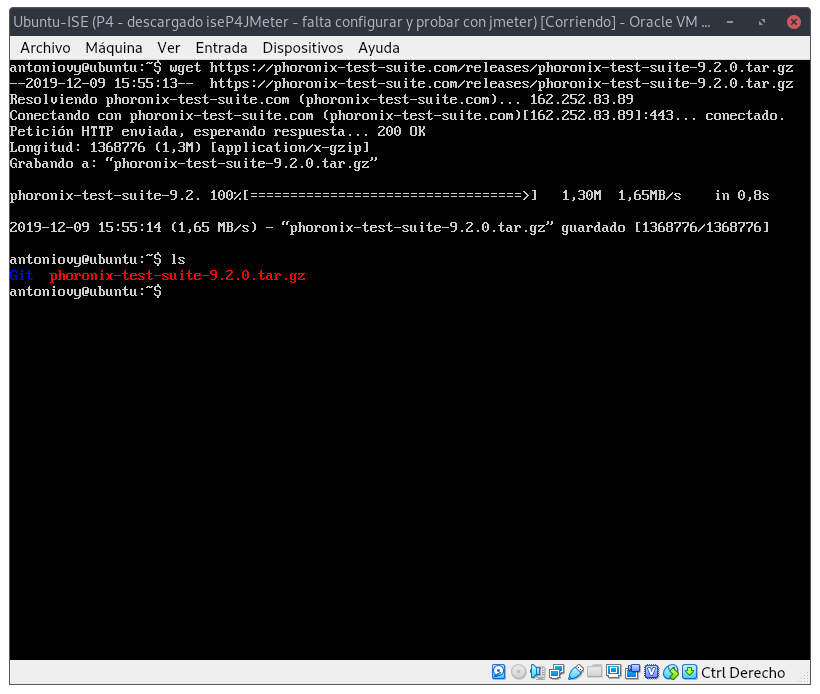
\includegraphics[scale=0.35]{descarga_pts.png}
\end{center}

\begin{center}
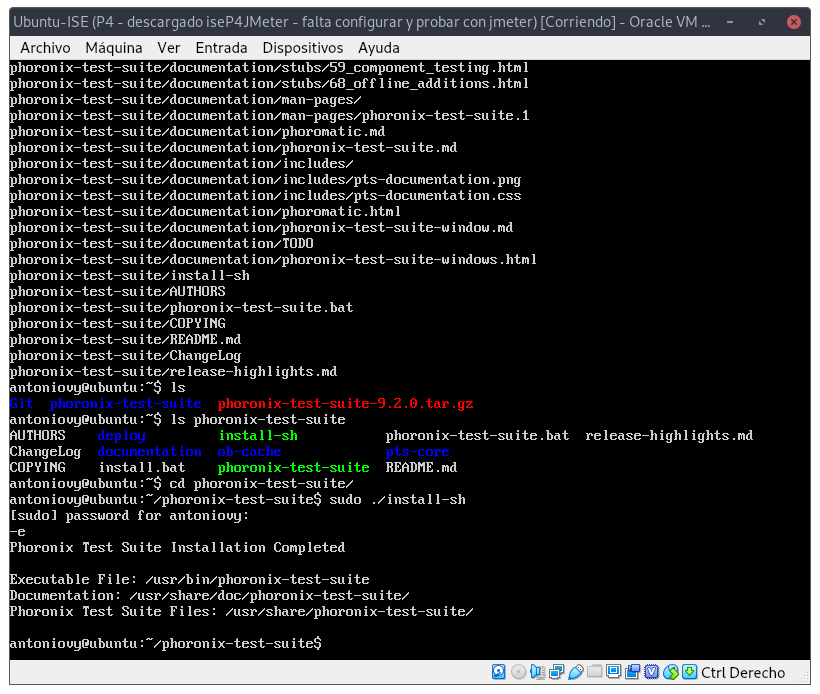
\includegraphics[scale=0.35]{instalacion_pts.png}
\end{center}


\subsection{Instalación en CentOS}

Al igual que con Ubuntu, descargamos el paquete y ejecutamos el script de instalación:

\begin{minted}[linenos,tabsize=2,breaklines]{bash}
\$ wget  https://phoronix-test-suite.com/releases/phoronix-test-suite-9.2.0.tar.gz
\$ tar -xvf phoronix-test-suite-9.2.0.tar.gz
\$ cd phoronix-test-suite/
\$ sudo ./install-sh
\end{minted}


\subsection{Instalación con Docker}

Otra opción es instalar Phoronix Test Suite a través de Docker\cite{pts_docker}

\begin{minted}[linenos,tabsize=2,breaklines]{bash}
\$ docker pull phoronix/pts
\end{minted}

Y ejecutarlo con:

\begin{minted}[linenos,tabsize=2,breaklines]{bash}
\$ docker run -it phoronix/pts
\end{minted}



\subsection{Ejecución de pruebas}

Una vez instalado, podremos realizar pruebas con la siguiente orden:

\begin{minted}[linenos,tabsize=2,breaklines]{bash}
\$ phoronix-test-suite benchmark <nombre_prueba>
\end{minted}

Algunas de las pruebas que he realizado y veremos más adelante son apache (benchmark que utiliza AB), php y smallpt (pequeña prueba para el procesador)


\subsection{Configuración de Phoromatic}

En mi caso ejecutaré el servidor de Phoromatic desde mi anfitrión con la ayuda del manual de phoronix-test-suite\cite{pts_man}.

Para configurar Phoromatic debemos incluir algunas extensiones de PHP, editando el archivo /etc/php/php.ini

\begin{minted}[linenos,tabsize=2,breaklines]{bash}
\$ sudo vim /etc/php/php.ini
\end{minted}

Y descomentamos las extensiones \texttt{sockets}, \texttt{sqlite3} y \texttt{zip}.


Con esto podemos pasar a ejecutar el servidor de Phoromatic con la siguiente orden:

\begin{minted}[linenos,tabsize=2,breaklines]{bash}
\$ phoronix-test-suite start-phoromatic-server
\end{minted}


\begin{center}
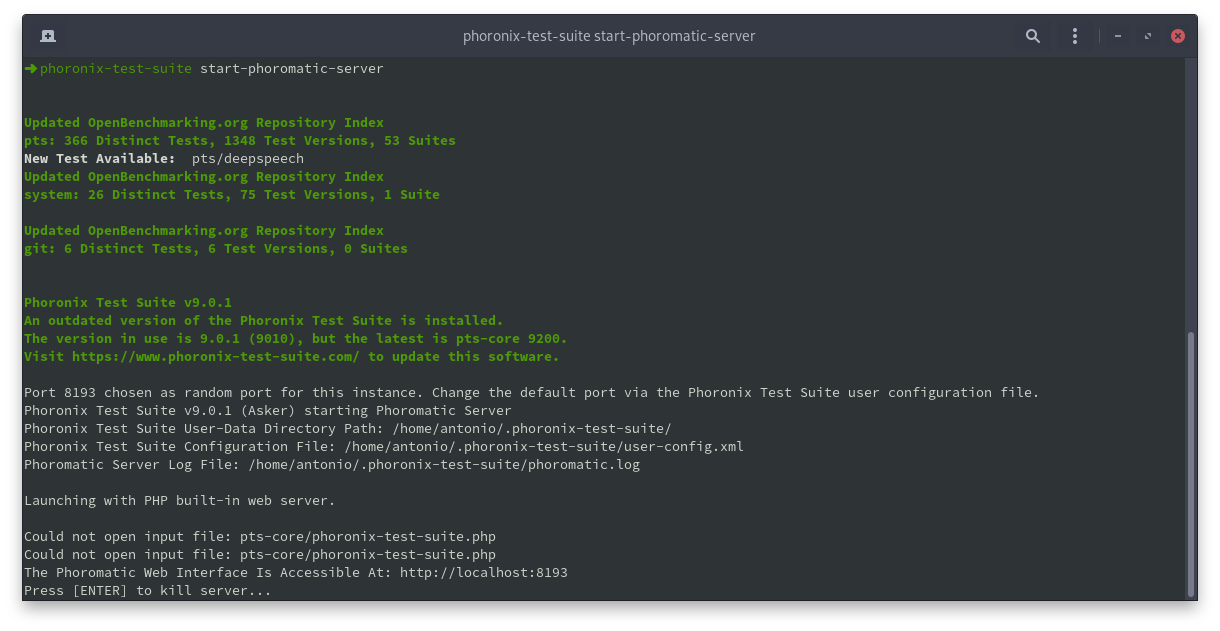
\includegraphics[scale=0.35]{phoromatic_server.png}
\end{center}


\subsection{Uso de Phoromatic}

Como podemos ver en la imagen anterior, podemos acceder a Phoromatic a través de la ruta\\ \texttt{http://localhost:8193}. Cada vez que iniciemos el servidor Phoromatic nos asignará un puerto, a no ser que especifiquemos un puerto en concreto en el archivo de configuración ubicado en\\ \texttt{$\textasciitilde$/.phoronix-test-suite/}

Al entrar en dicha URL nos pedirá un login:

\begin{center}
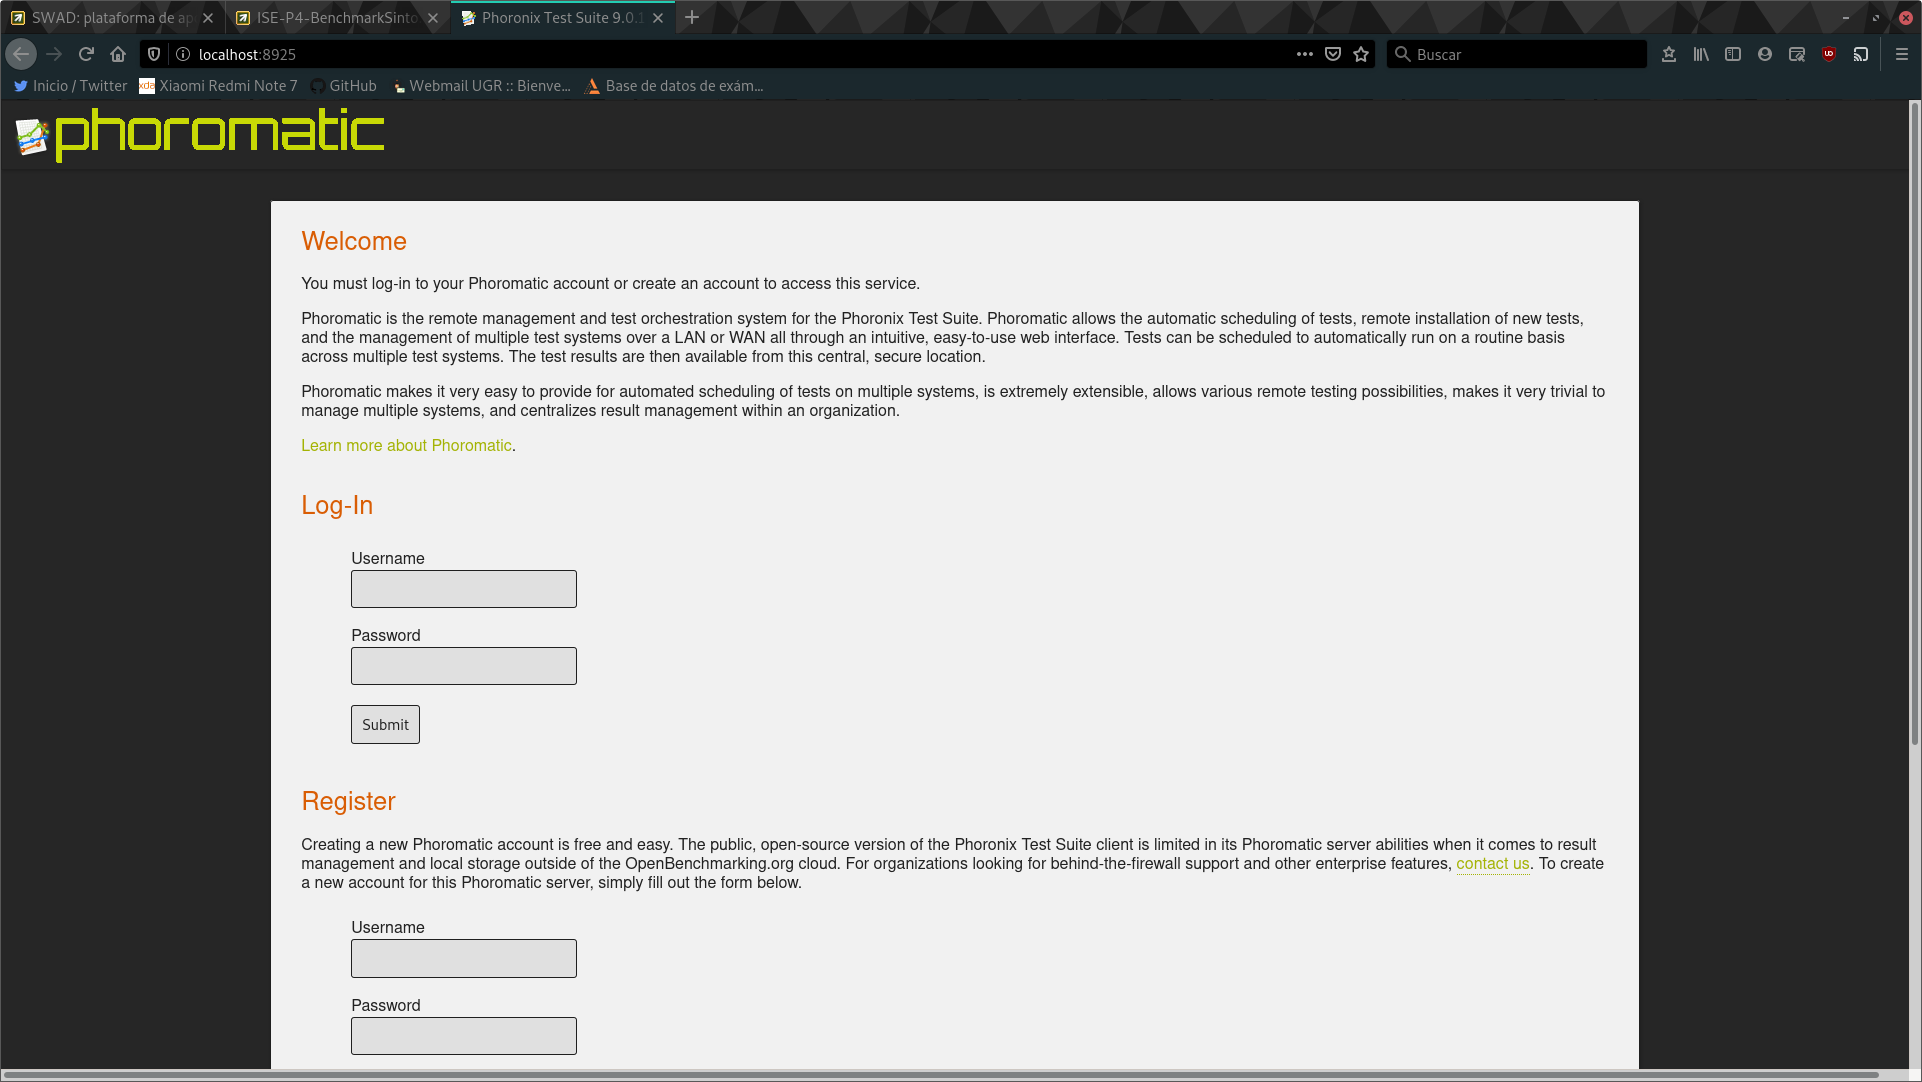
\includegraphics[scale=0.25]{login_phoromatic.png}
\end{center}

Tras registrarnos, encontraremos la siguiente página:

\begin{center}
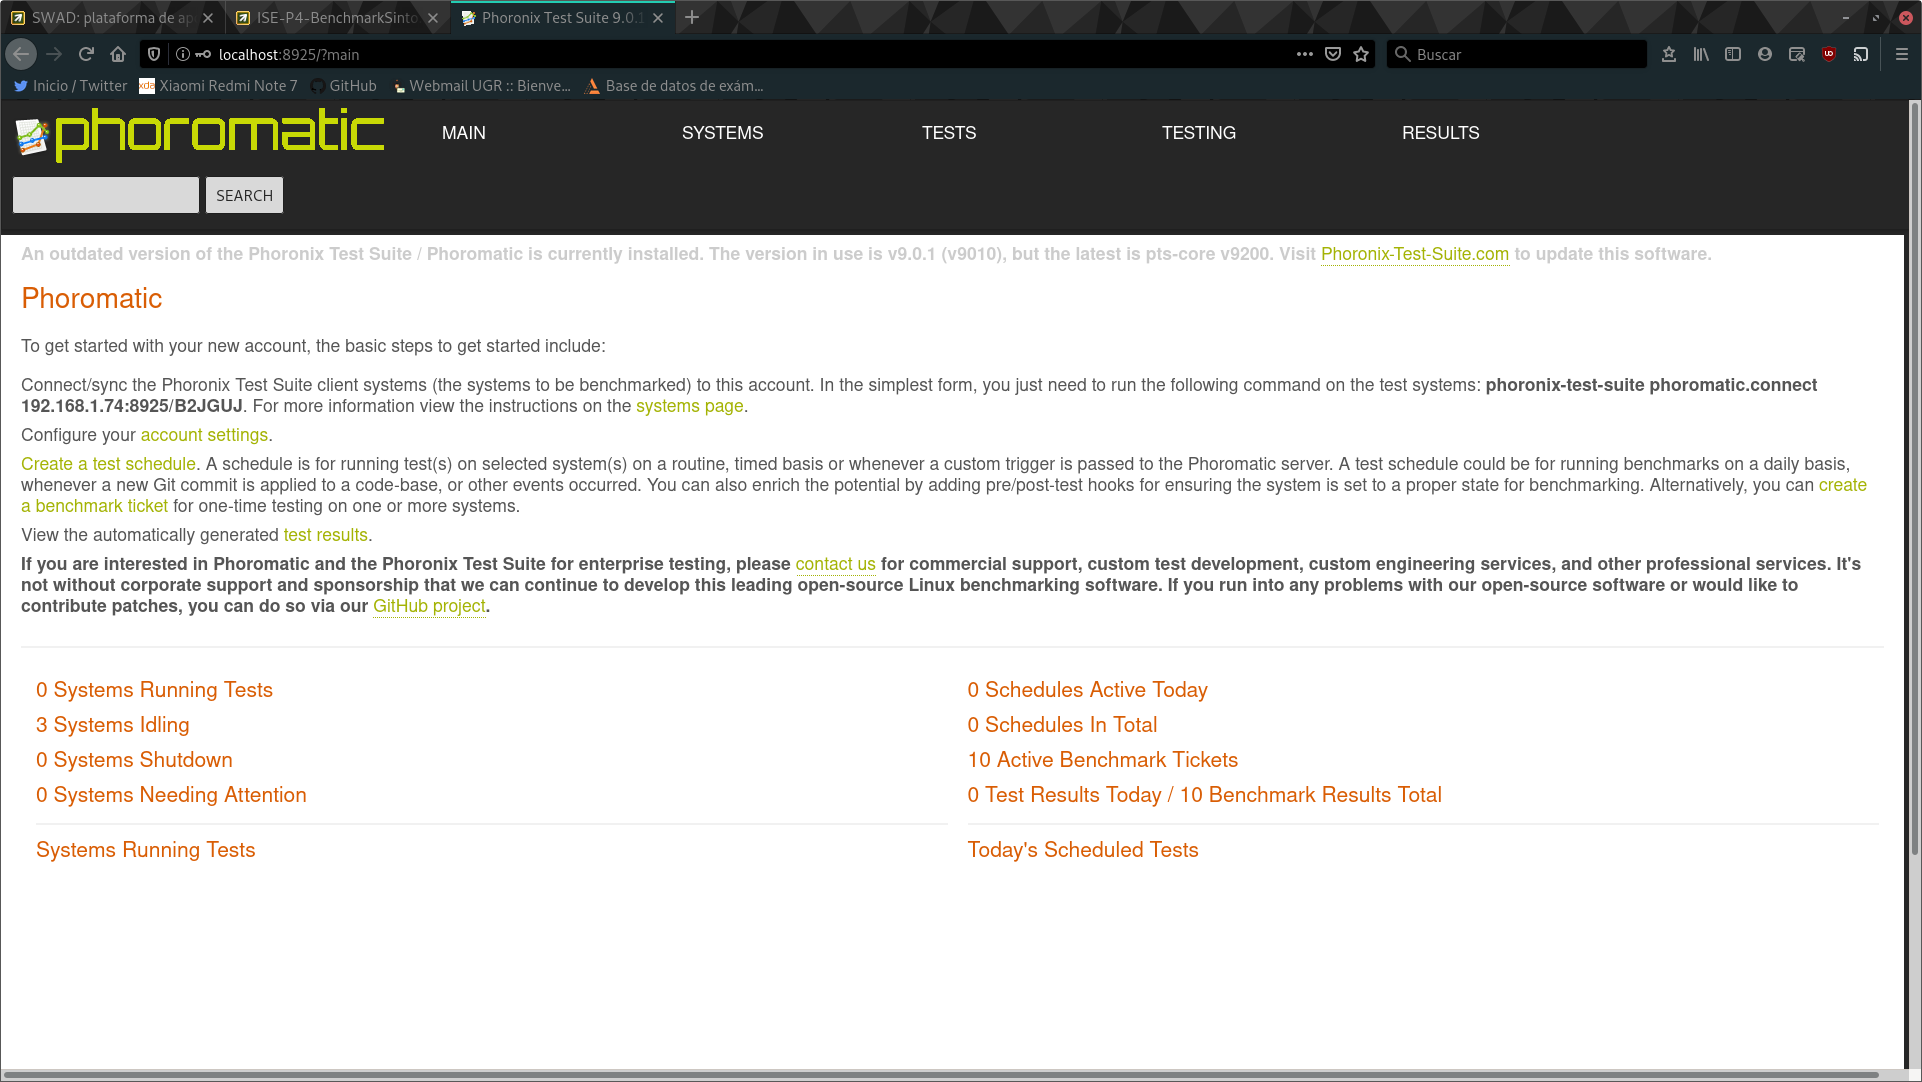
\includegraphics[scale=0.25]{main_phoromatic.png}
\end{center}

En mi caso aparecen tres máquinas, ya que tengo añadidos los tres sistemas.

\subsubsection{Añadir y conectar equipos a Phoromatic}

Como vemos en la última imagen, añadir o conectar un sistema es tan sencillo como ejecutar el comando que nos indica el servidor:

\begin{minted}[linenos,tabsize=2,breaklines]{bash}
\$ phoronix-test-suite phoromatic.connect 192.168.1.74:8925/B2JGUJ
\end{minted}

La ruta puede variar cada vez que iniciemos el servidor (a excepción de fijar una en los archivos de configuración), mientras que la última parte de la URL es un identificador único asociado al usuario de Phoromatic.

La primera vez que añadimos un equipo nos preguntará que nombre queremos asignarle dentro del servidor de Phoromatic. En mi caso los equipos se llaman CentOS-ISE, Ubuntu-ISE y antonio, siendo los dos primeros las máquinas virtuales de la asignatura y el último mi anfitrión.

En la pestaña de sistemas de Phoromatic podemos ver los sistemas que tenemos conectados, y cuando fue su ultima conexión. (La tasa de refresco es de aproximadamente uno a dos minutos.)

\begin{center}
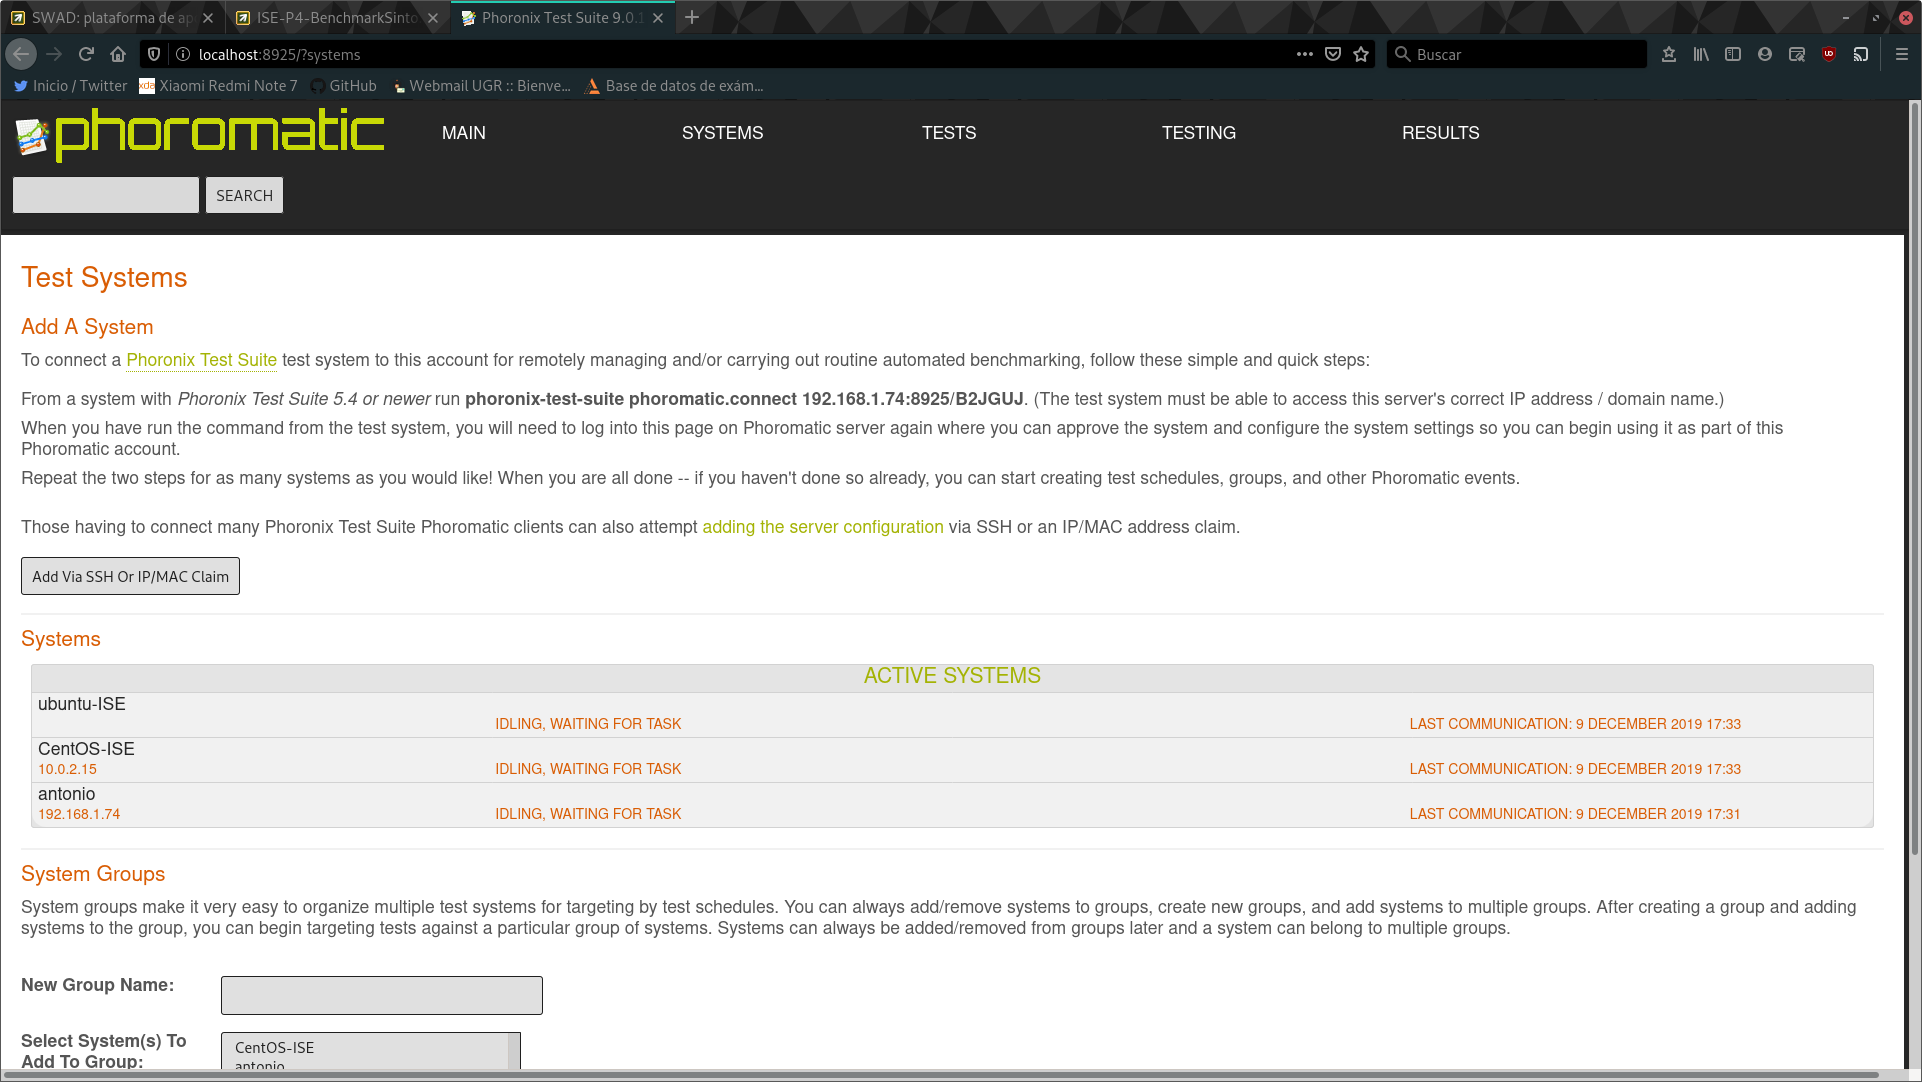
\includegraphics[scale=0.25]{phoromatic_systems.png}
\end{center}

\subsubsection{Crear Tests Suites}

En la pestaña Tests podemos crear perfiles de test, así como nuevas suites personalizadas, en nuestro caso, vamos a crear una suite que tenga como test SmallPT:

\begin{center}
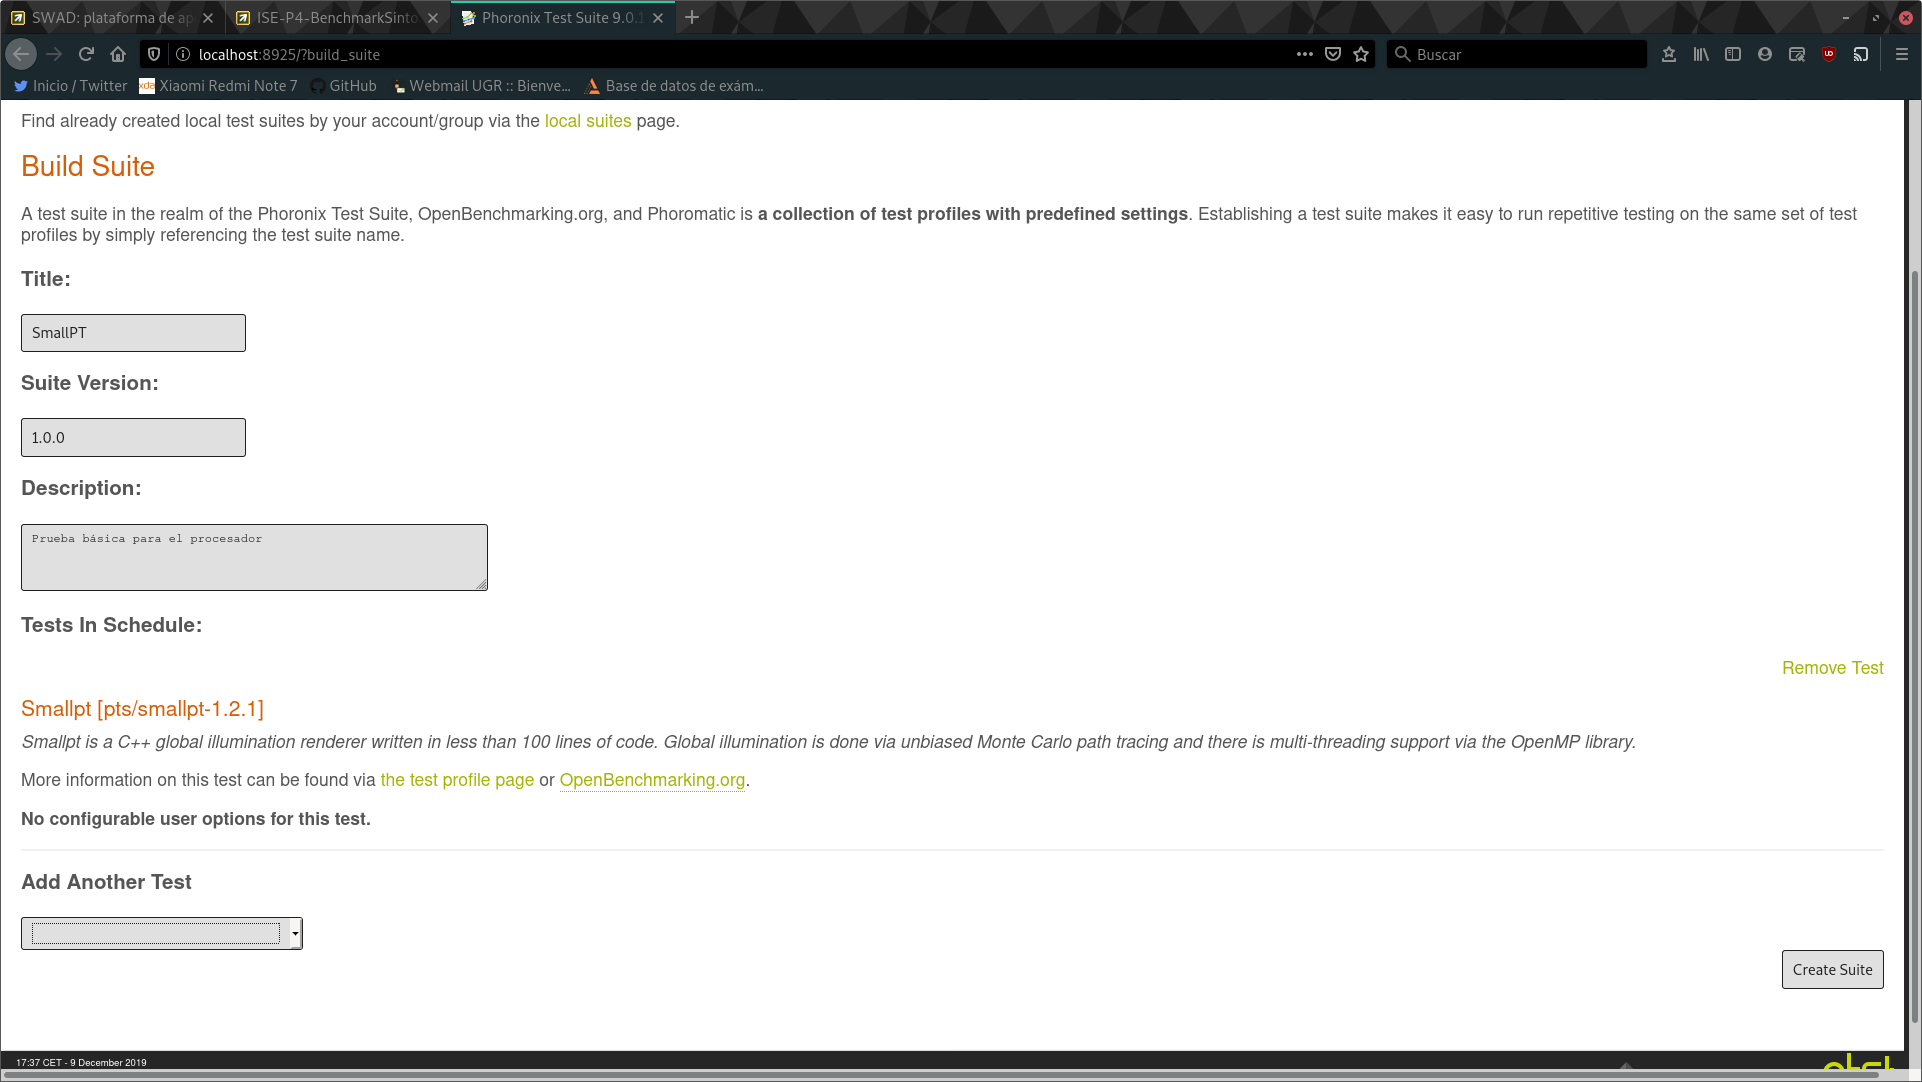
\includegraphics[scale=0.25]{phoromatic_suite.png}
\end{center}

Como vemos, podemos hacer que una suite ejecute un conjunto de tests, por si queremos, por ejemplo, aplicar distintos tests de CPU a un equipo, sin tener que ejecutarlos uno a uno manualmente.

\subsubsection{Ejecutar Suites}

En la sección Testing tenemos disponible la opción Run a benchmark, donde podemos escoger que suite ejecutar y en que sistemas ejecutarlos. En mi caso, al estar virtualizando dos de los sistemas en el anfitrión solo mandaré las pruebas a un único host simultaneamente, sin embargo, si fueran servidores distintos podríamos mandar simultaneamente suites a ejecutar.

\begin{center}
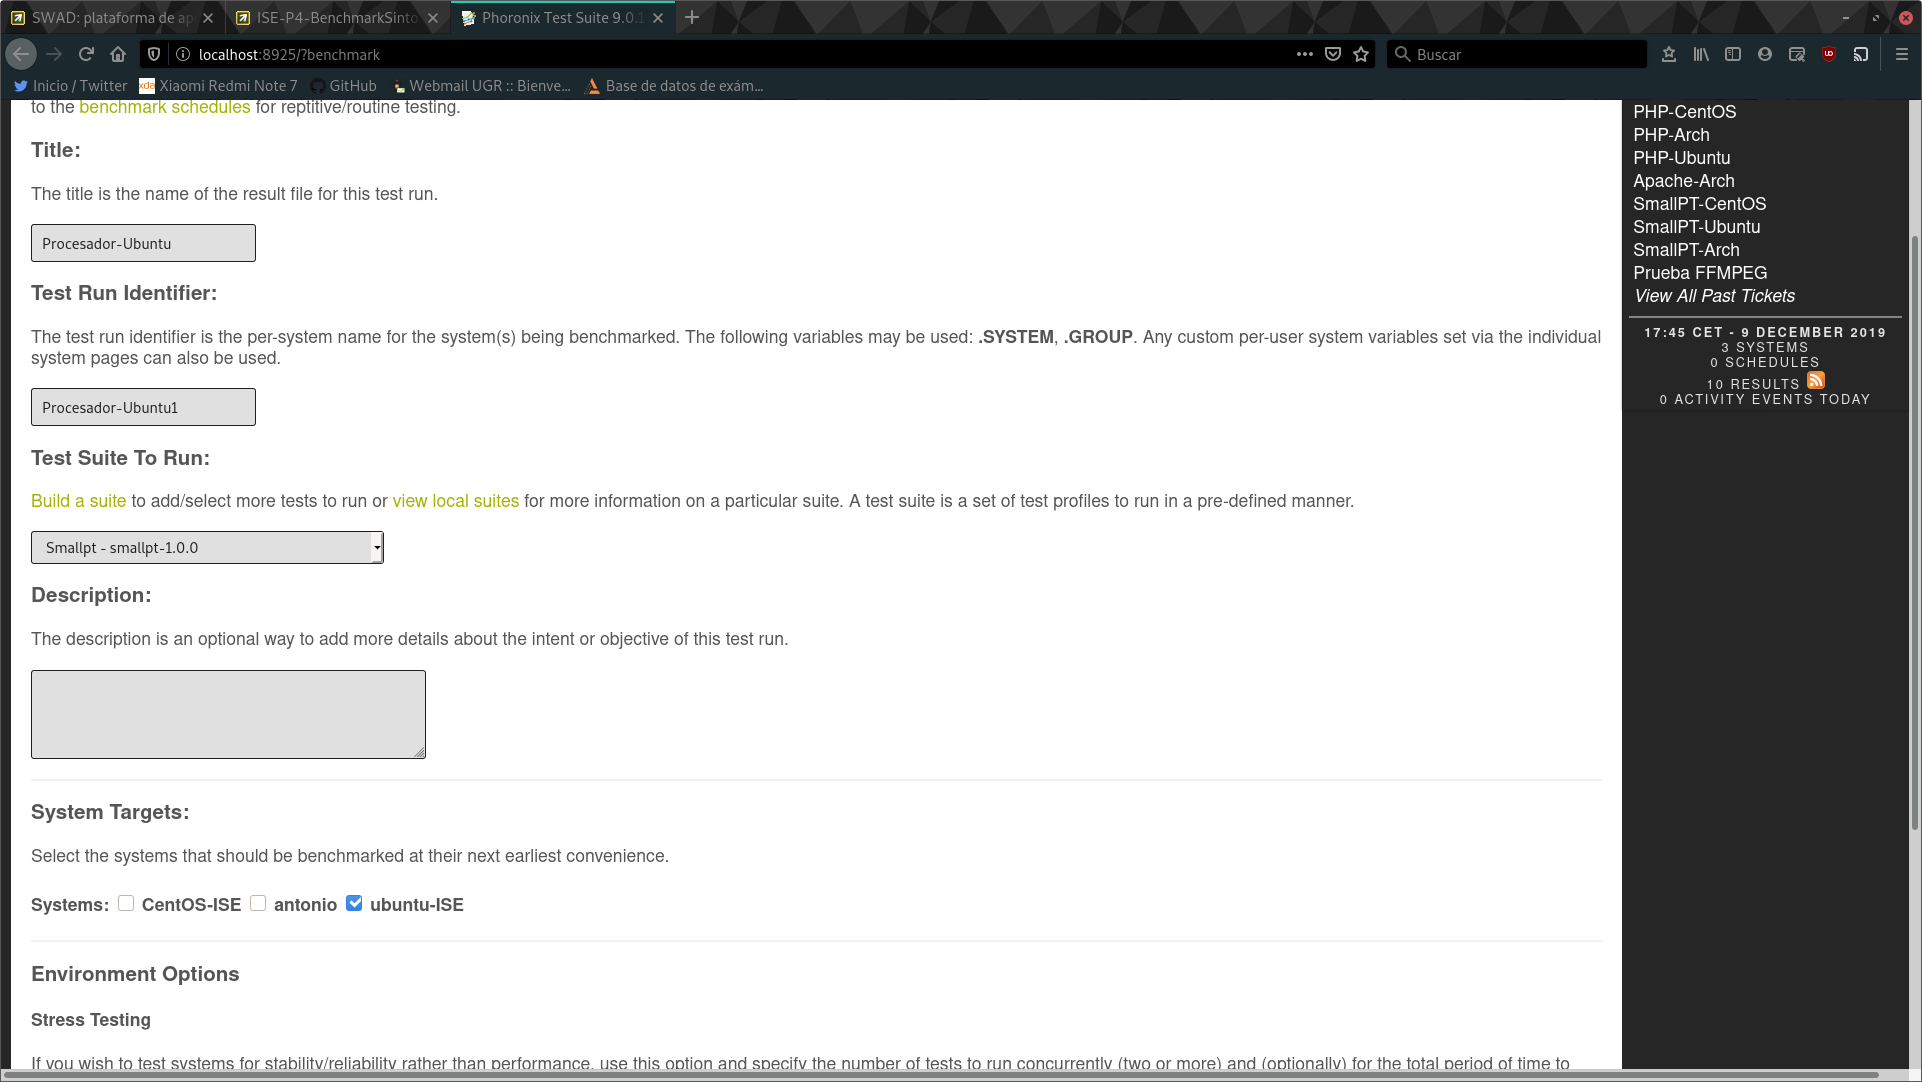
\includegraphics[scale=0.25]{phoromatic_exec.png}
\end{center}


\newpage
Vemos como también nos permite establecer el numero de concurrencia, así como el tiempo mínimo que estará ejecutando el test.

\begin{center}
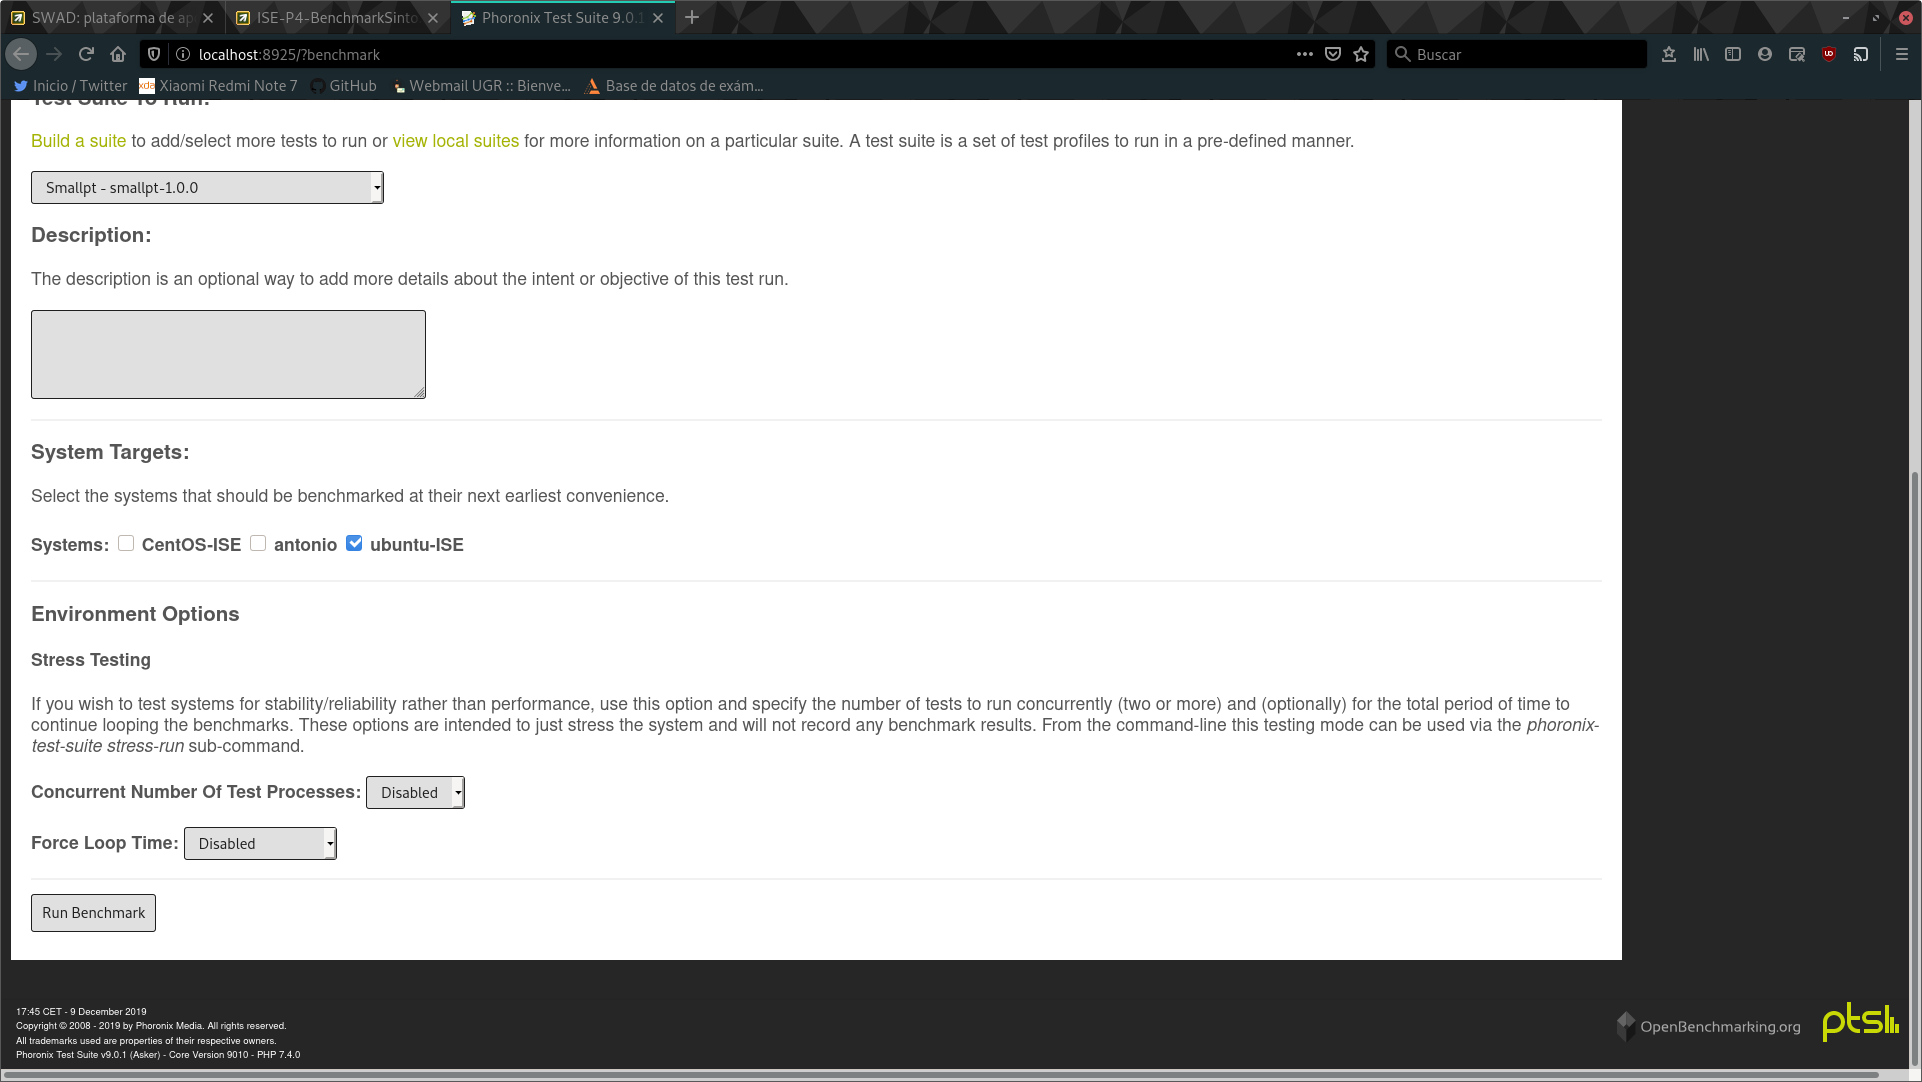
\includegraphics[scale=0.25]{phoromatic_exec2.png}
\end{center}


Una vez mandamos el benchmark, phoronix-test-suite se encargará de instalarlo, ejecutarlo, y devolver los resultados a Phoromatic.

\begin{center}
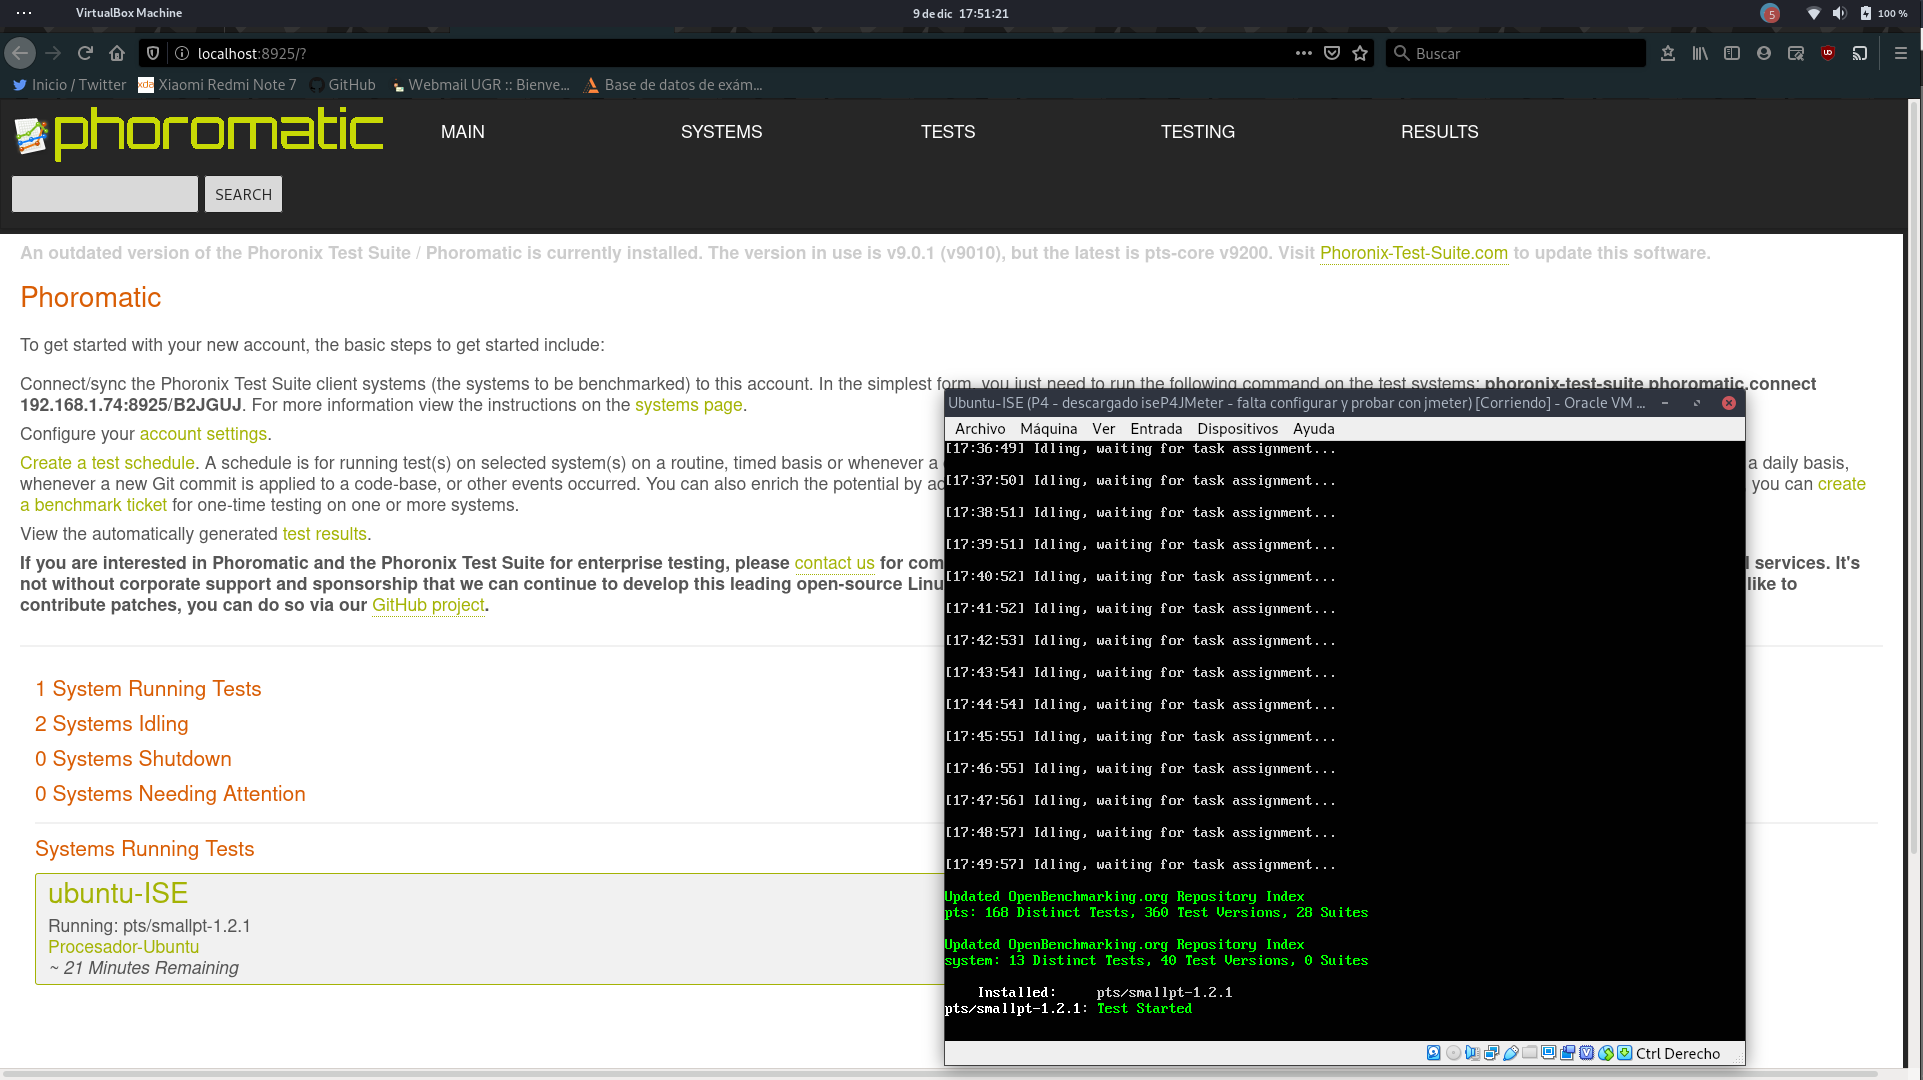
\includegraphics[scale=0.25]{phoromatic_ejecucion.png}
\end{center}


\subsubsection{Mostrar resultados}

En la opción de Results tenemos disponibles los distintos resultados:

\begin{center}
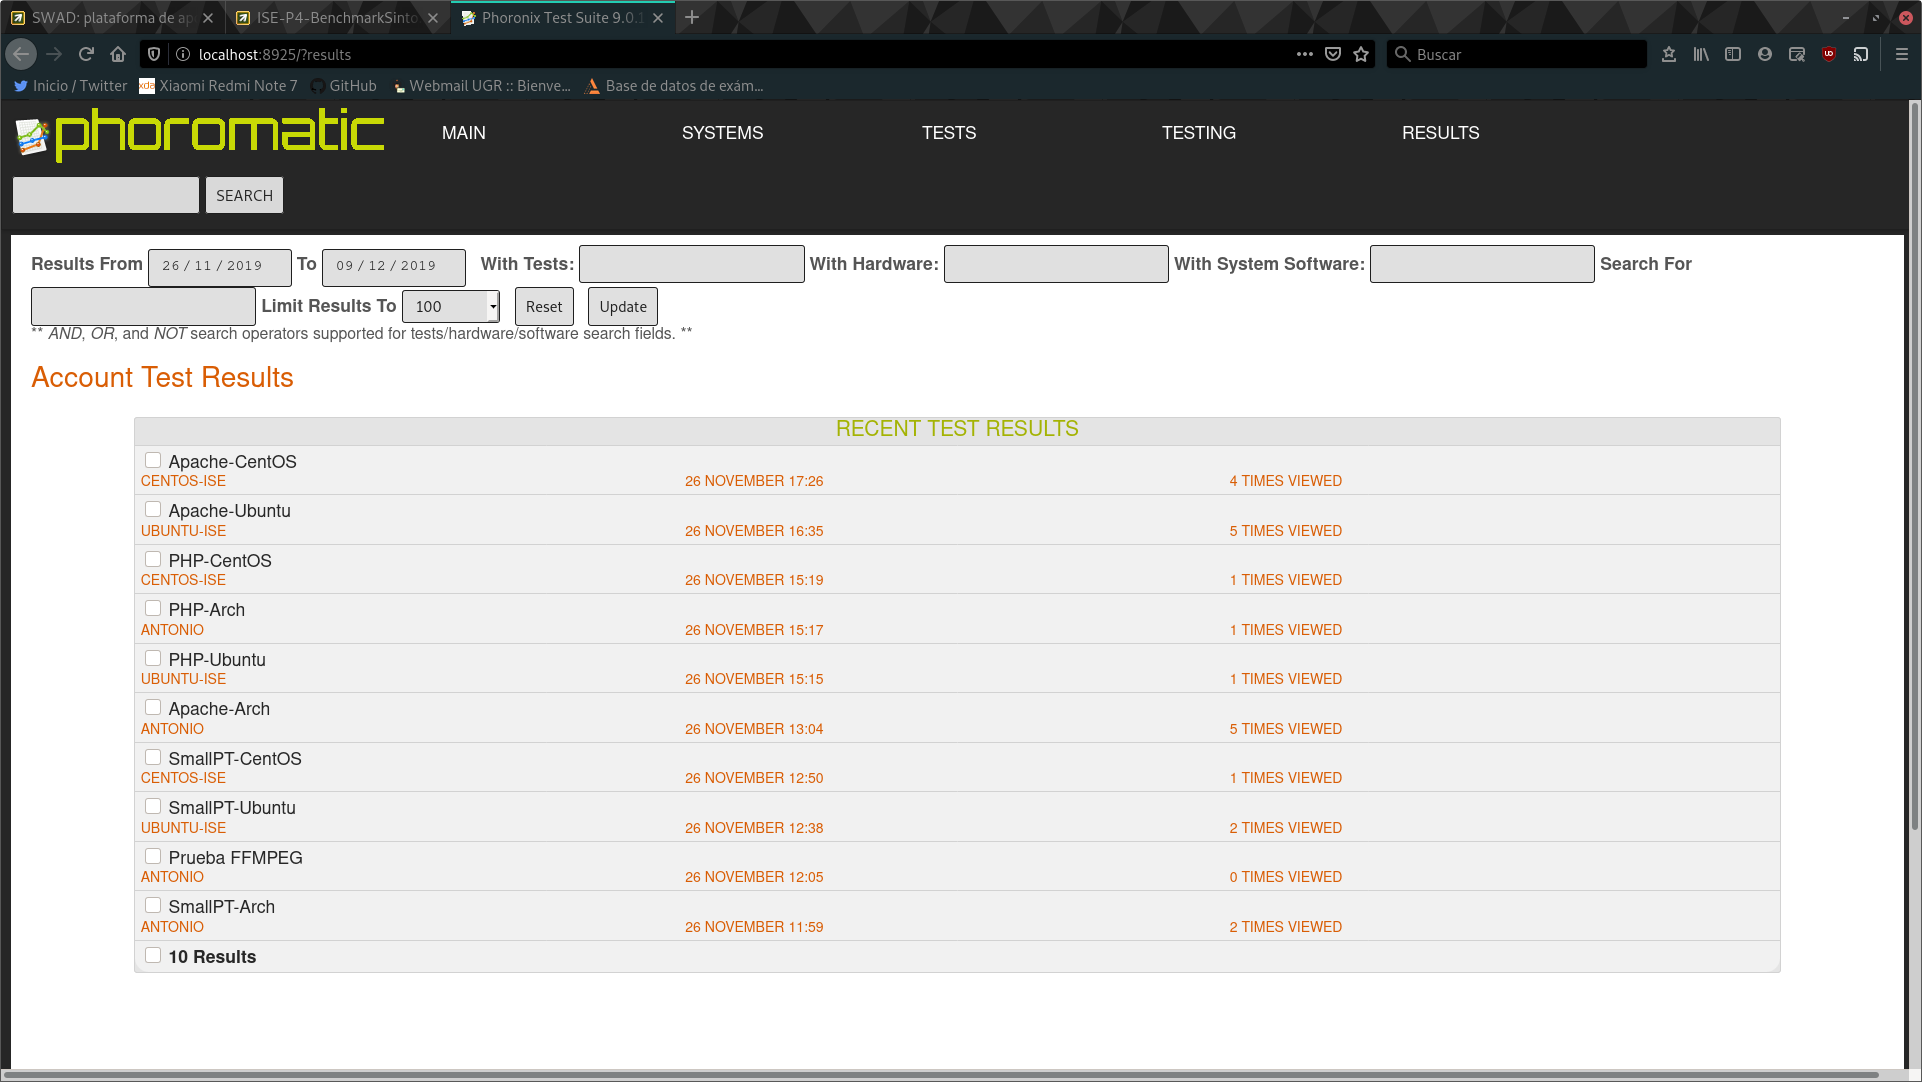
\includegraphics[scale=0.25]{phoromatic_results.png}
\end{center}

Podemos escoger varios (o solo uno) y compar los resultados, pinchando en la nueva opción del menú: Compare


\begin{center}
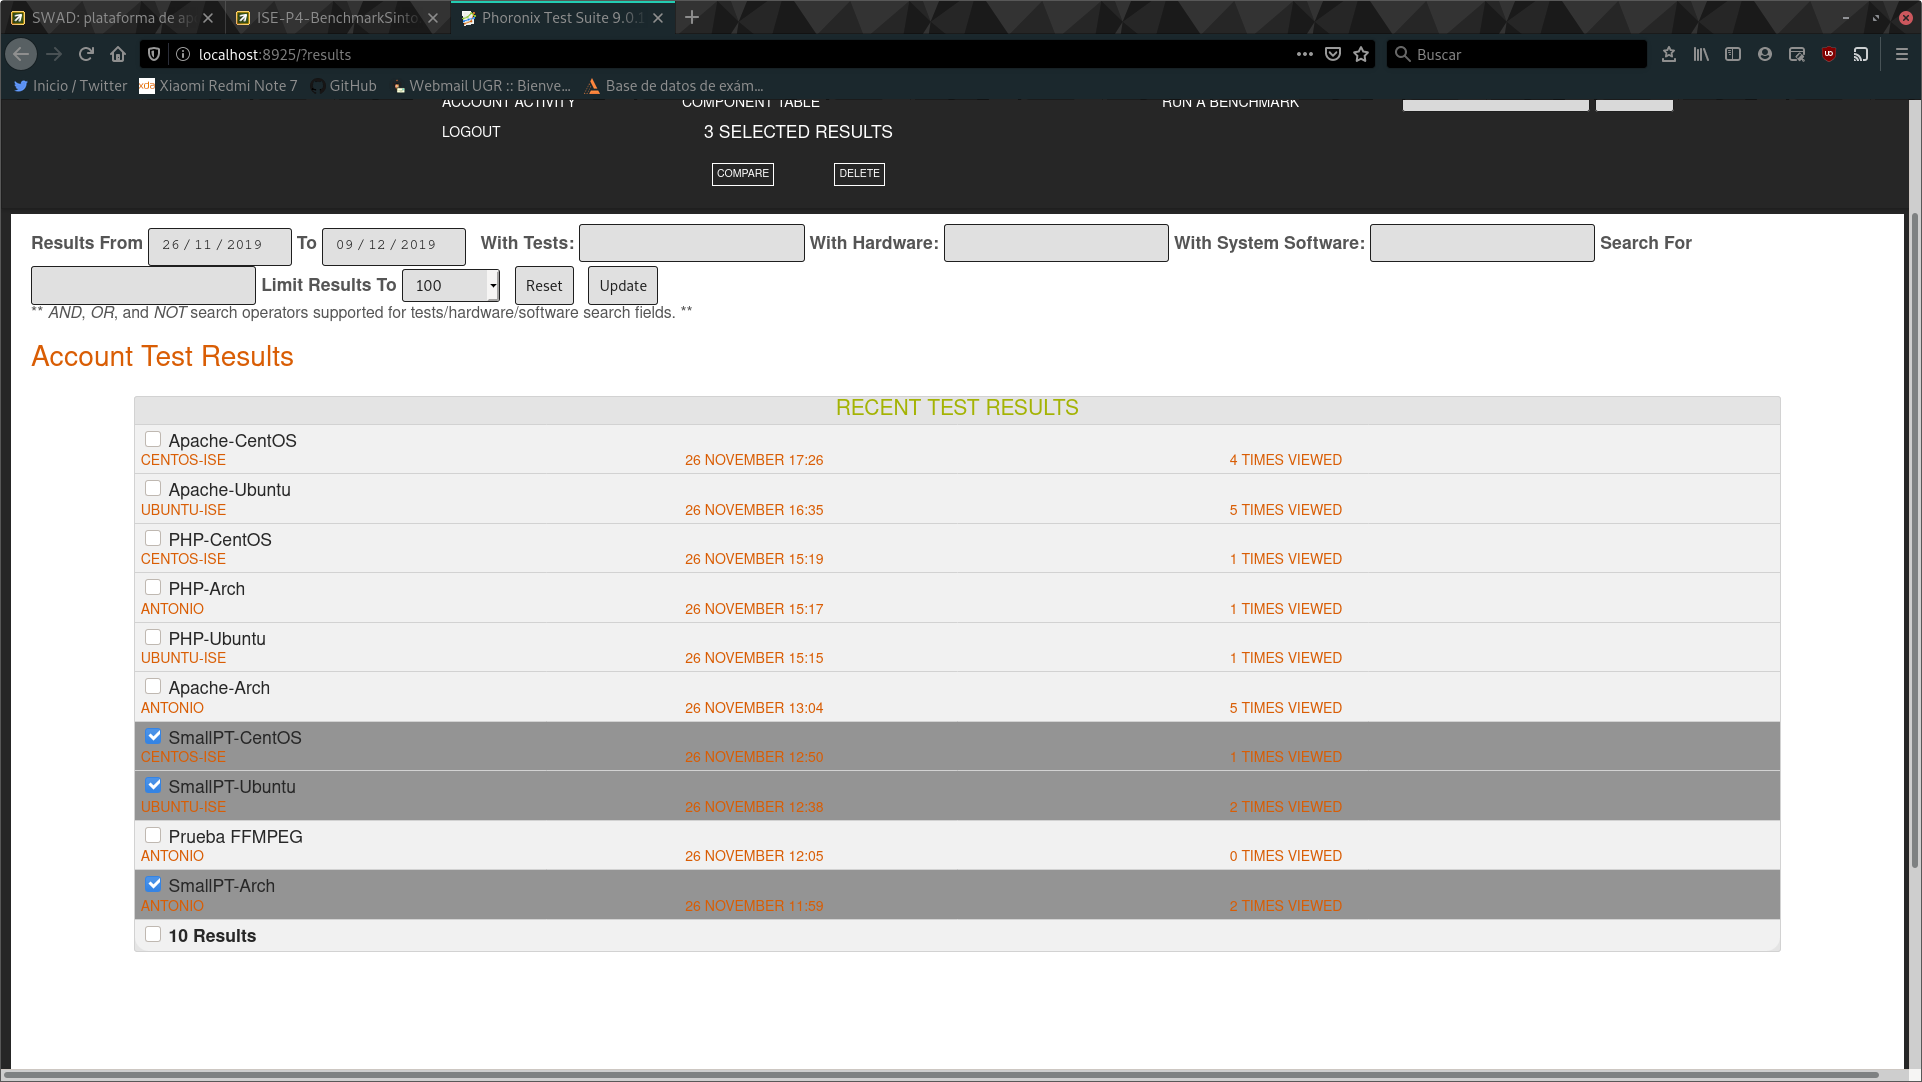
\includegraphics[scale=0.25]{phoromatic_compare.png}
\end{center}

Nos aparecerá esta pestaña, donde tenemos información de cada sistema, así como los resultados:

\begin{center}
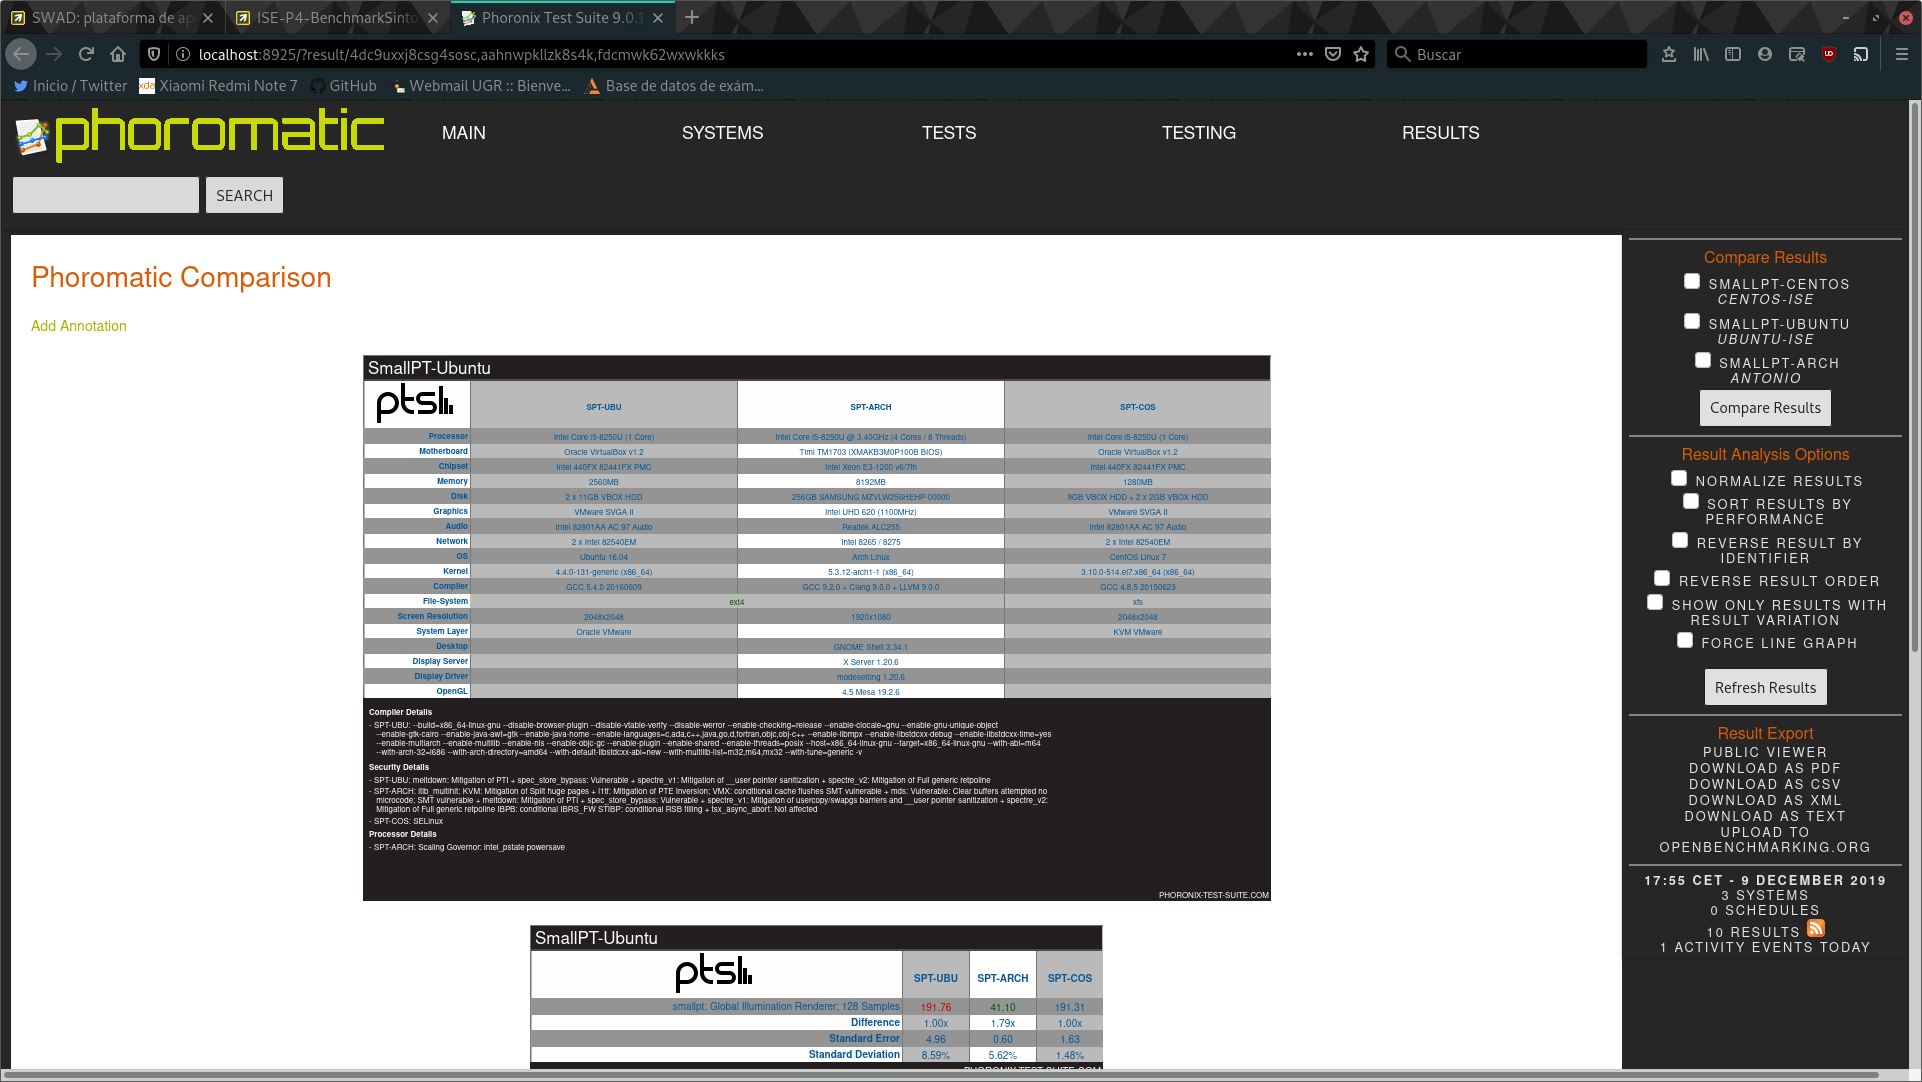
\includegraphics[scale=0.25]{phoromatic_datos.png}
\end{center}

\begin{center}
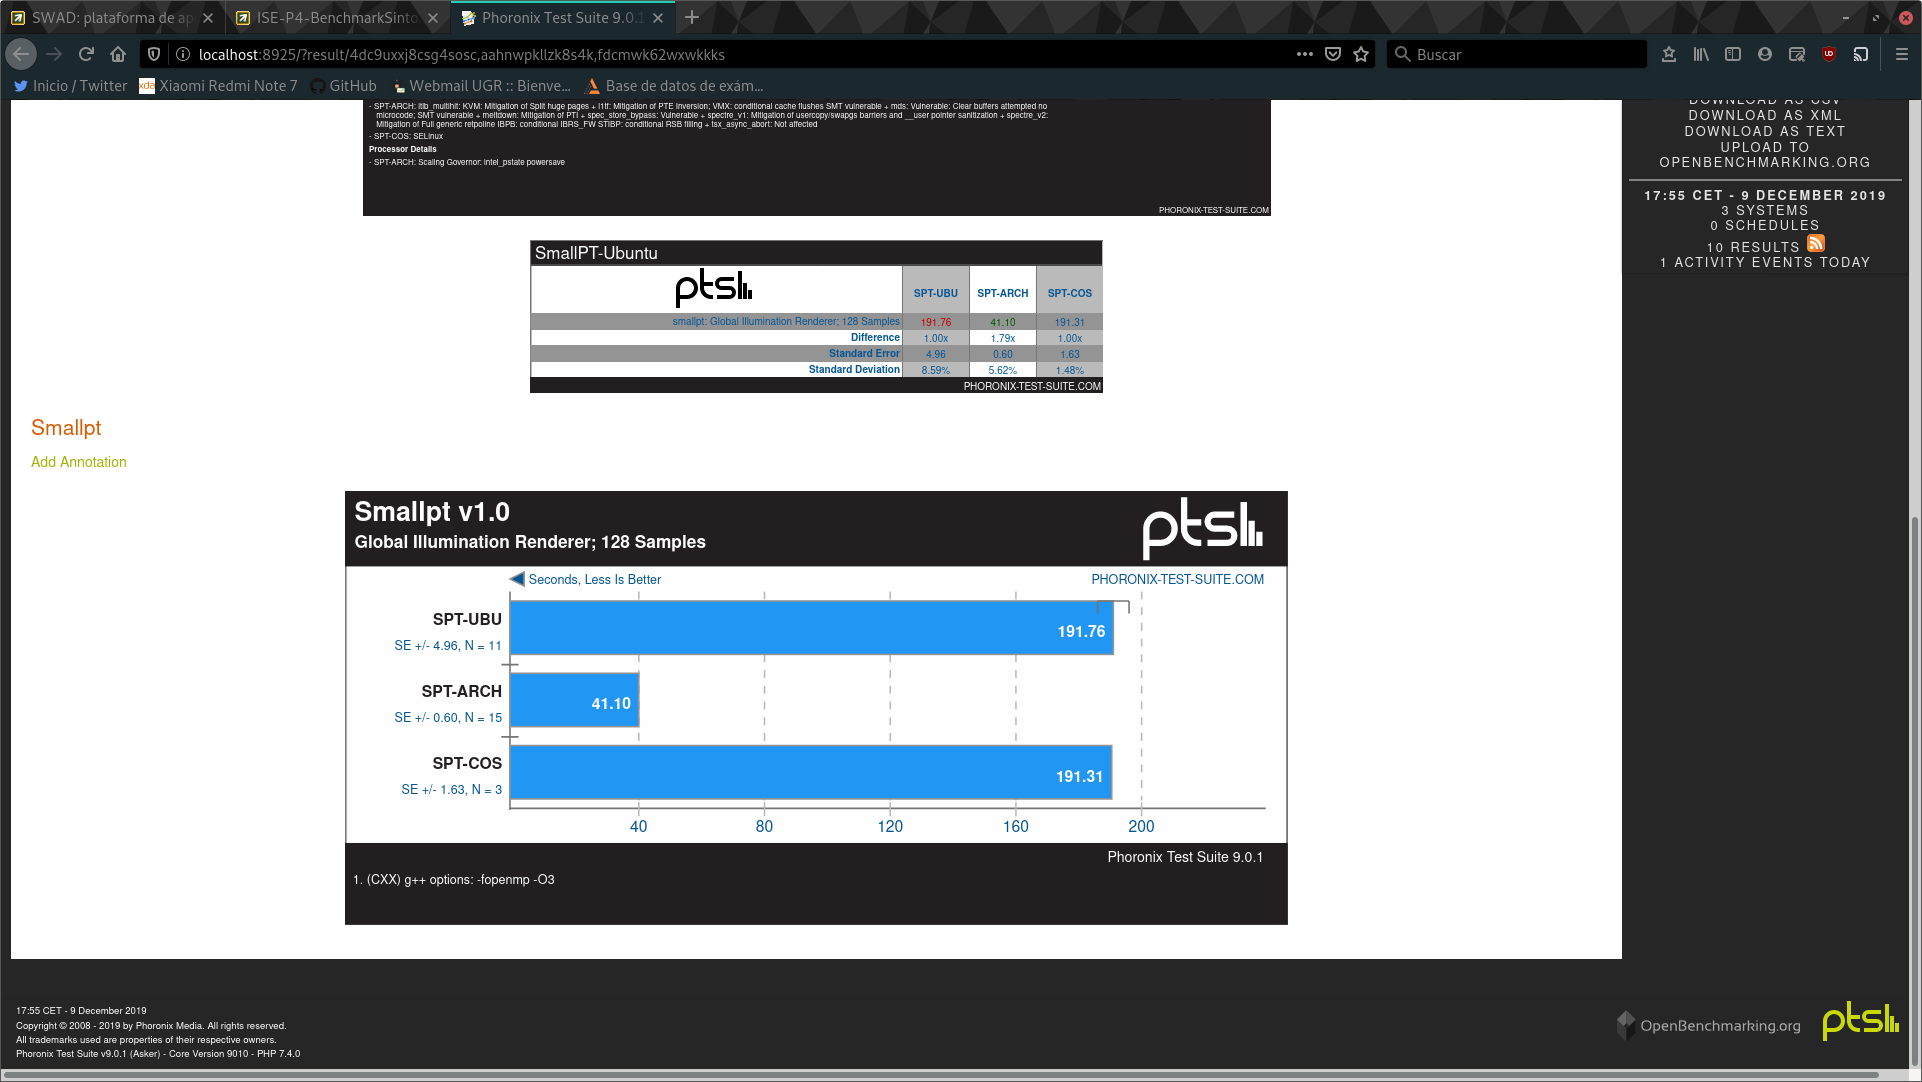
\includegraphics[scale=0.25]{phoromatic_graph.png}
\end{center}

\section{Apache AB}

Apache AB (Apache Benchmark) es un software diseñado y distribuido por Apache para comprobar y medir el rendimiento del servicio Apache, es decir, medir cuantas peticiones es capaz de servir nuestro servidor con Apache instalado. 

\subsection{Instalación de Apache AB}

AB es instalado junto a Apache, esto quiere decir que en los equipos usados, al instalar \texttt{apache2} en el caso de Ubuntu Server o \texttt{httpd} en el caso de CentOS el software AB ya es instalado automáticamente.

\subsection{Uso de AB}

Como vemos en la documentación oficial de AB\cite{ab_doc} tenemos distintas opciones para usar AB, desde opciones para hacer login en caso de que el servidor este protegido, protocolo de seguridad a usar, manejo de cookies, carga de datos desde archivos csv entre muchas otras opciones.

Nosotros nos centraremos en las opciones \texttt{-n} y  \texttt{-c}:

\begin{itemize}
	\item \textbf{Opción \texttt{-n}}: Con este parámetro podemos establecer el número de peticiones que se van a realizar al servidor. Su valor por defecto es 1, por lo que no suele ser representativo y no es suficiente para obtener un benchmark realista.
	
	\item \textbf{Opción \texttt{-c}}: Número de peticiones concurrentes, es decir, el número de peticiones que se realizarán a la vez. Su valor por defecto es 1.
\end{itemize}



También cabe mencionar que aunque exista la opción \texttt{-c} no existe un paralelismo real, es decir, nuestra máquina solo ejecutará una instancia de AB en la que realizará muchas peticiones por segundo, pero el asignar un número N de concurrencia no significa ejecutar N instancias de AB. Sin embargo, para el servidor si serán peticiones distintas, por lo que tendrá que generar una instancia de apache por cada petición.

\begin{center}
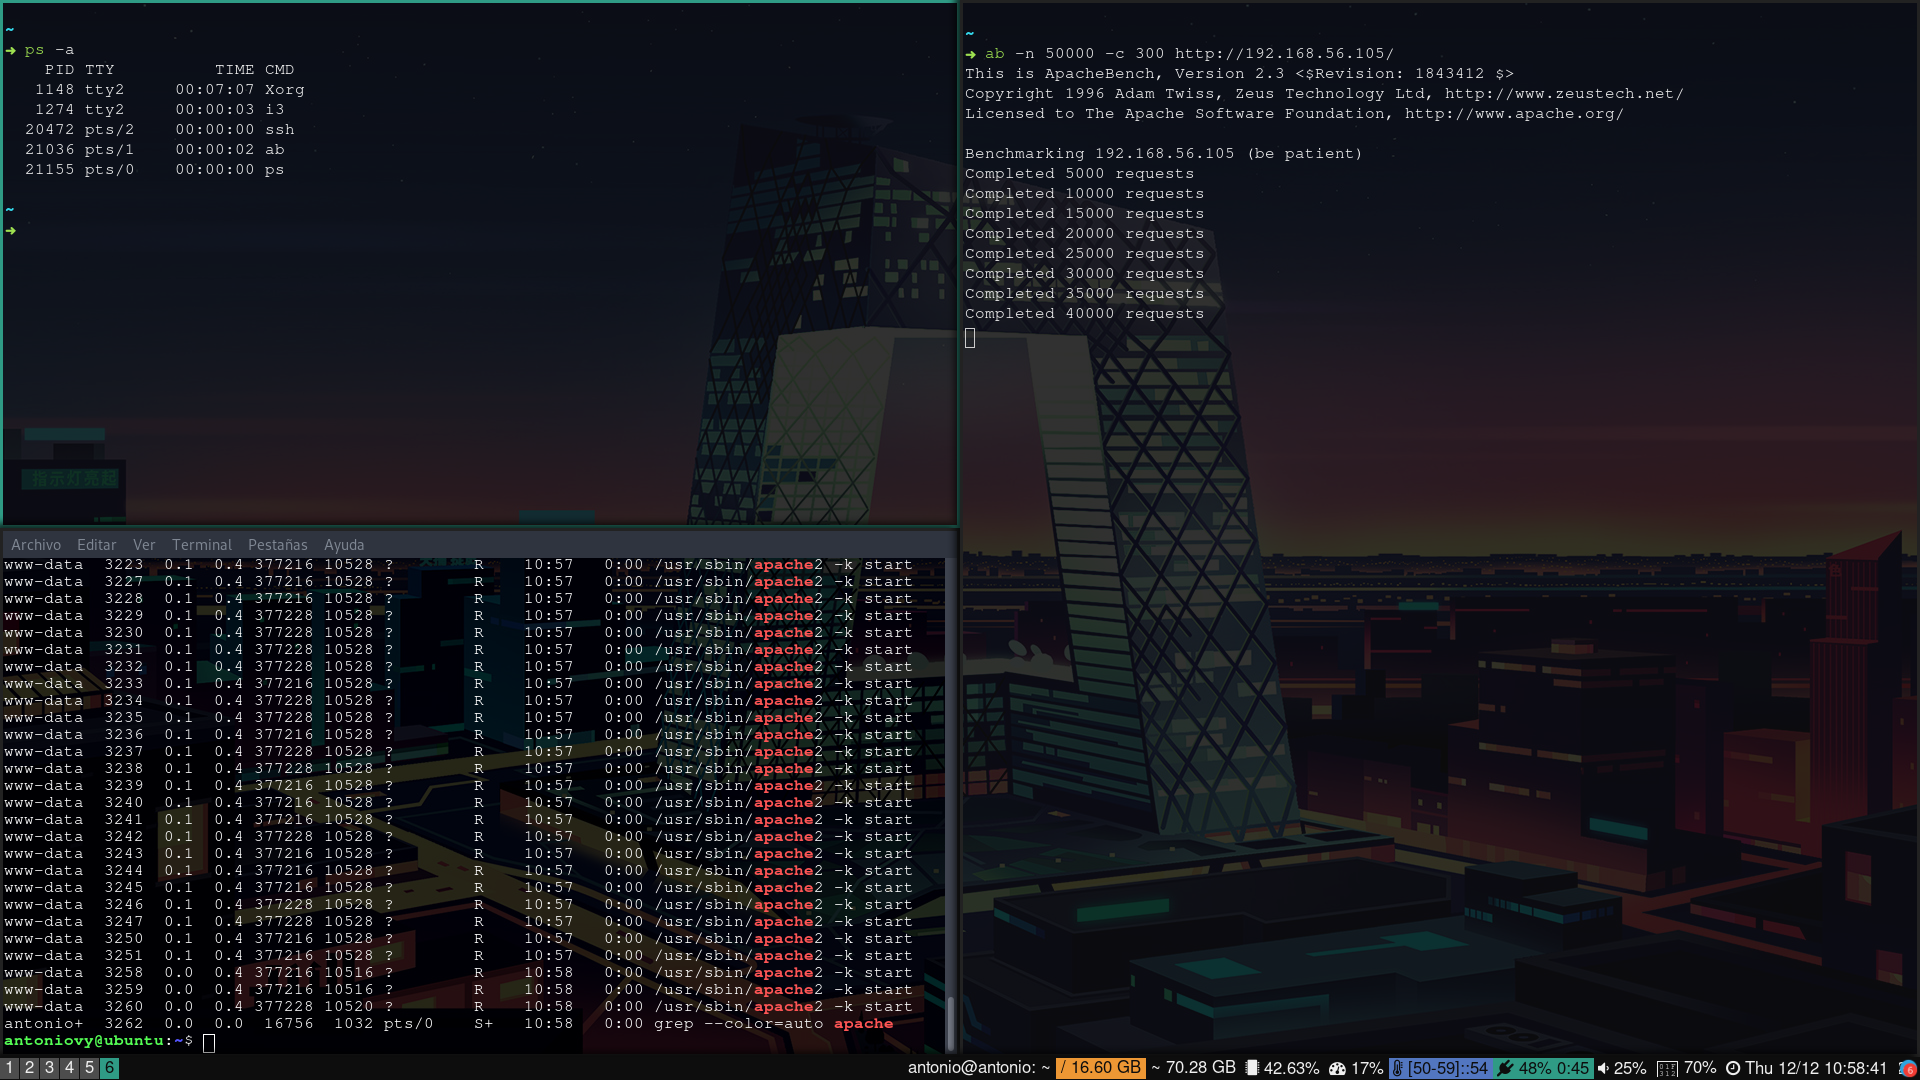
\includegraphics[scale=0.25]{test-ab.png}
\end{center}

\newpage

\subsection{Interpretar la salida de AB}

La ejecución de AB nos dará la siguiente salida:


\begin{center}
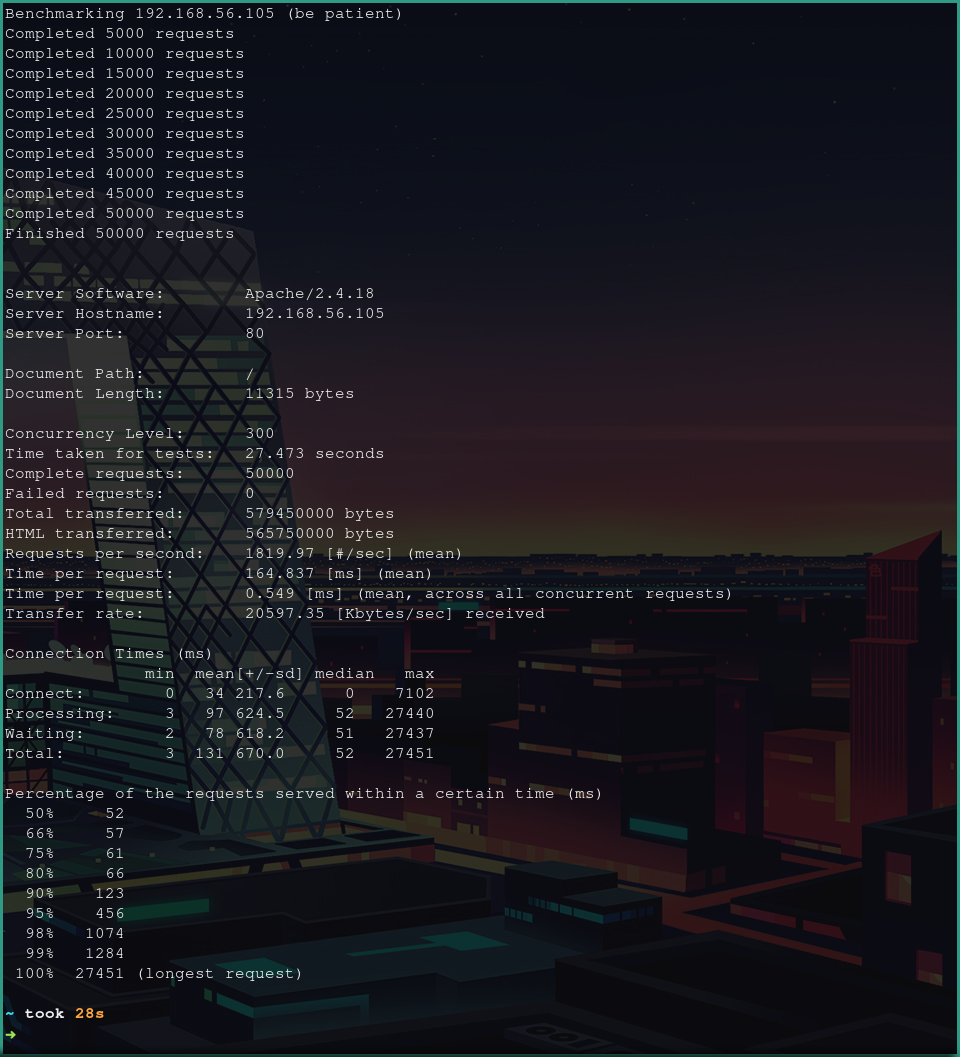
\includegraphics[scale=0.45]{salida-ab.png}
\end{center}

Como vemos en la documentación de AB\cite{salida_ab} la salida de AB se compone de:

\begin{enumerate}
	\item Información sobre el servidor (Server Software, Server Hostname y Server Port), en nuestro caso el servidor ejecuta una versión de Apache 2.4.18, el hostname es 192.168.56.105 y estamos accediendo a través del puerto 80.
	\item Información sobre el documento solicitado(Document Path y Document Length). El documento solicitado se encuentra en la ruta / (raíz) del servidor Apache, y tiene una longitud de 11315 bytes.
	\item Nivel de concurrencia. Corresponde al parámetro \texttt{-c} pasado en la ejecución de AB. Por defecto vale 1.
	\item Tiempo que ha necesitado el test. En nuestro 27.473 segundos.
	\item Peticiones completadas. En nuestro ejemplo 50.000, es decir, todas.
	\item Peticiones fallidas. En nuestro ejemplo 0.
	\item Total de datos transferidos. En nuestro caso 579.450.000 bytes.
	\item HTML transferido. En nuestro caso 565.750.000 bytes, que corresponden a la longitud del documento por el número de peticiones.
	\item Media de peticiones por segundo. En nuestro Apache ha servido una media de 1819.97 peticiones por segundo.
	\item Tiempo medio por petición (secuencial). En nuestro ejemplo 164.837 ms.
	\item Tiempo medio por petición (concurrente). En nuestro ejemplo 0.549 ms.
	\item Velocidad de transmisión. En nuestro ejemplo 20597 KBytes/segundo.
	\item Tiempos de conexión. Nos muestra los tiempos medios de conexión, procesado, espera y el total.
	\item Porcentaje de peticiones servidas a los T milisegundos. Normalmente esta medición la haremos con el 99\% de las peticiones, es decir, la mayoría de estas.
\end{enumerate}


\newpage

\subsection{Comparación CentOS y Ubuntu Server}

Para realizar esta prueba he clonado el archivo \texttt{index.html} por defecto de Apache en Ubuntu Server en CentOS, asegurando que el tamaño de bytes a transferir es el mismo, para poder realizar una prueba fiable.


\begin{center}
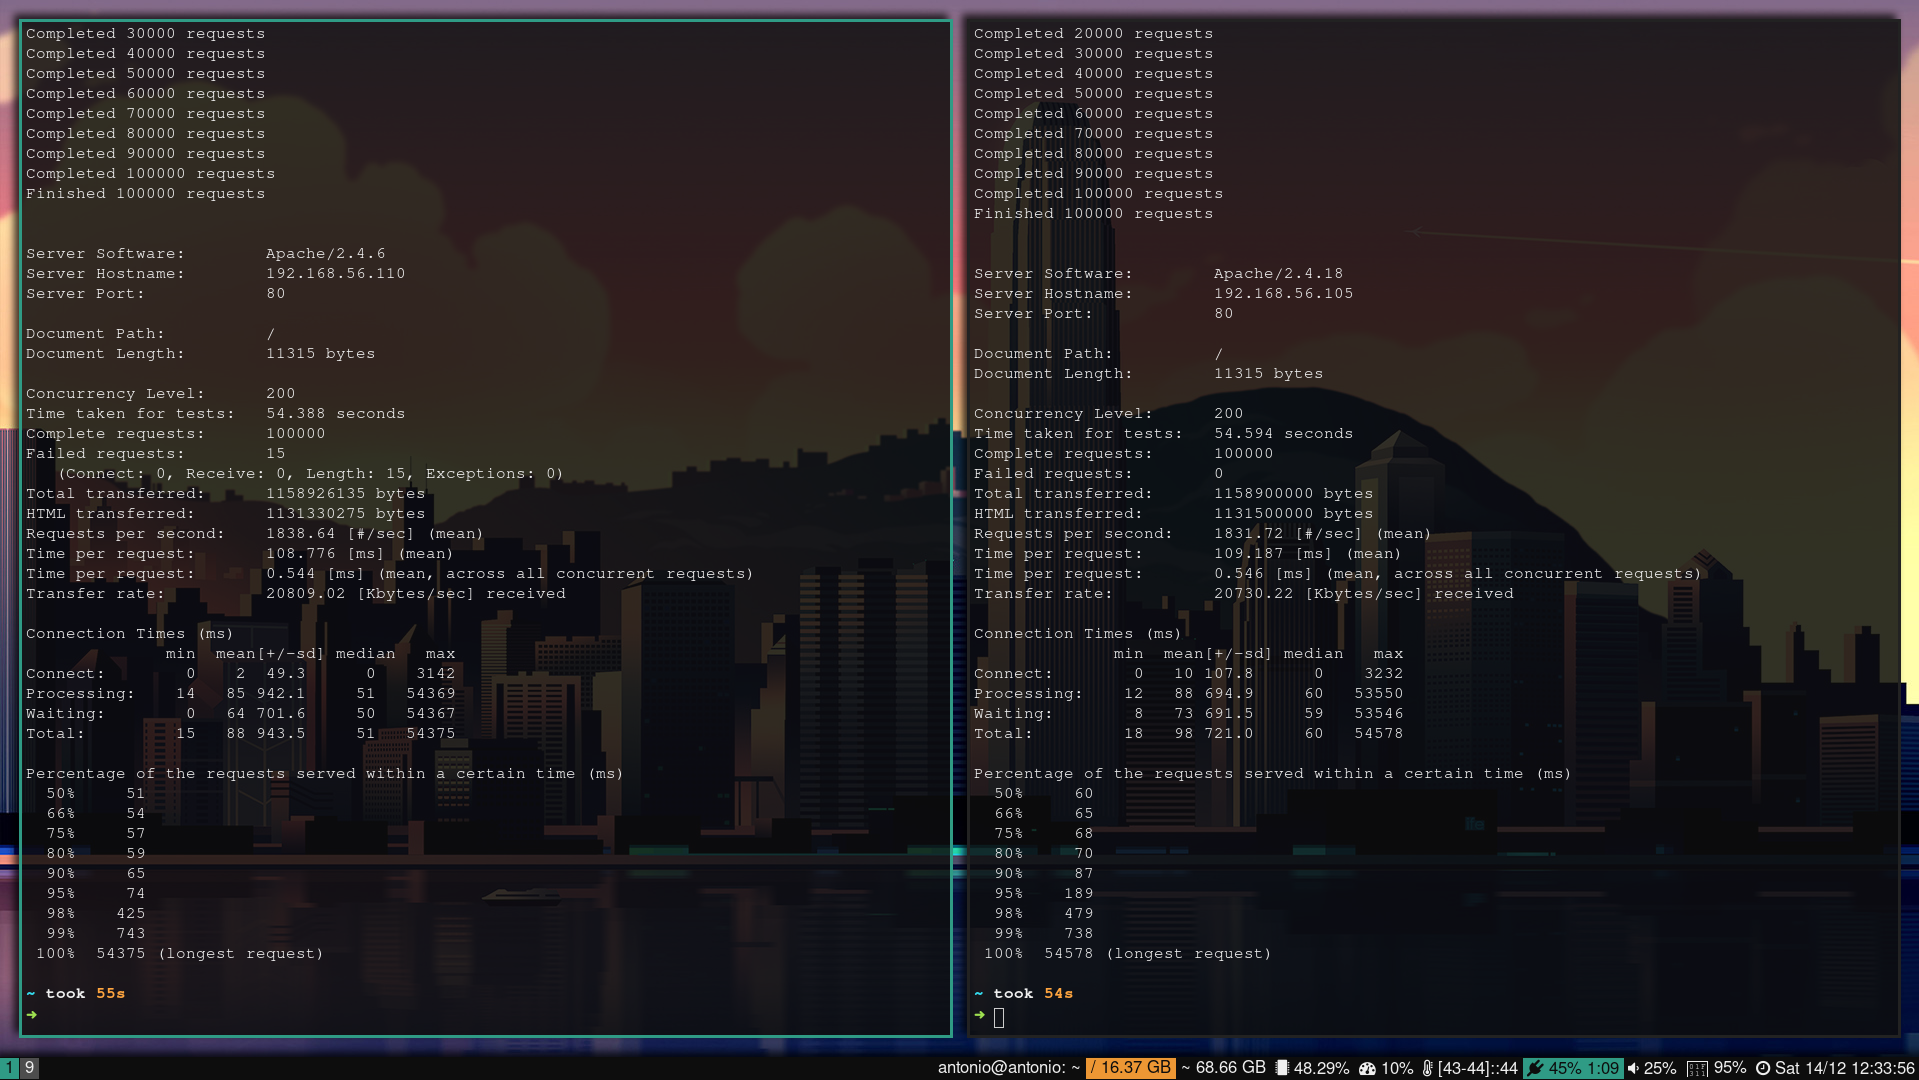
\includegraphics[scale=0.25]{ab-ubu-cent.png}
\end{center}

Vemos como el número de bytes transferidos es el mismo, tanto en el total como en HTML.

De esta comparación podemos obtener que CentOS es ligeramente más rápido al debido al tiempo de servicio de las peticiones, sin embargo esta prueba es demasiado pequeña ya que únicamente transferimos un archivo HTML básico.

\newpage

\section{JMeter}

JMeter\cite{main_jmeter} es un proyecto desarrollado por Apache con el objetivo de desarrolar una herramienta de prueba de carga para analizar y medir el desempeño tanto de un servidor como de los servicios que este pueda ofrecer.

\subsection{Instalación de JMeter}

Para instalar JMeter en mi anfitrión (ArchLinux) podemos instalarlo desde el AUR (Arch User Repository)

\begin{minted}[linenos,tabsize=2,breaklines]{bash}
\$ yay -S jmeter 
\end{minted}

En CentOS y Ubuntu no será necesario instalar JMeter, ya que las peticiones las haremos desde nuestro anfitrión.

\subsection{Instalando el microservicio iseP4JMeter}

Para realizar la práctica se nos pide usar un microservicio dado por lo profesores de la asignatura\cite{iseP4JMeter}.

Para usar este microservicio debemos instalar primero docker y docker-compose.

\subsubsection{Instalación de Docker y Docker-compose en Ubuntu Server}

Siguiendo los pasos del guión de prácticas:

Primero debemos añadir la llave GPG de Docker a APT:

\begin{minted}[linenos,tabsize=2,breaklines]{bash}
\$ curl -fsSL https://download.docker.com/linux/ubuntu/gpg | sudo apt-key add - 
\end{minted}

Añadimos el repositorio de Docker:

\begin{minted}[linenos,tabsize=2,breaklines]{bash}
\$  sudo add-apt-repository "deb [arch=amd64] https://download.docker.com/linux/ubuntu \$(lsb_release -cs) stable"
\end{minted}


Actualizamos la lista de repositorios e instalamos Docker y Docker-compose:
\begin{minted}[linenos,tabsize=2,breaklines]{bash}
\$  sudo apt update
\$ sudo apt install docker-ce docker-compose
\end{minted}

Añadimos a nuestro usuario al grupo de docker:
\begin{minted}[linenos,tabsize=2,breaklines]{bash}
\$  sudo usermod -aG docker \$USER
\end{minted}

Tras esto ya tenemos todo lo necesario instalado, aunque para que esta última instrucción tenga efecto debemos cerrar y volver a abrir la sesión.


\subsubsection{Instalación de Docker y Docker-compose en CentOS}

En el guión de prácticas no encontraremos como instalar docker en CentOS, pero con una búsqueda rápida encontramos la documentación de Docker\cite{dockerCentOS}.

Instalamos el paquete \texttt{yum-utils} para gestionar los repositorios de yum:

\begin{minted}[linenos,tabsize=2,breaklines]{bash}
\$  sudo yum install -y yum-utils  device-mapper-persistent-data lvm2
\end{minted}


Añadimos el repositorio de Docker:

\begin{minted}[linenos,tabsize=2,breaklines]{bash}
\$  sudo yum-config-manager --add-repo https://download.docker.com/linux/centos/docker-ce.repo
\end{minted}


Instalamos Docker y Docker-compose:

\begin{minted}[linenos,tabsize=2,breaklines]{bash}
\$  sudo yum install docker-ce docker-compose
\end{minted}


Añadimos a nuestro usuario al grupo de docker:
\begin{minted}[linenos,tabsize=2,breaklines]{bash}
\$  sudo usermod -aG docker \$USER
\end{minted}

Activamos y ejecutamos el servicio de Docker:
\begin{minted}[linenos,tabsize=2,breaklines]{bash}
\$  sudo systemctl start docker
\$ sudo systemctl enable docker
\end{minted}


Tras esto ya tenemos Docker y Docker-compose instalado.


\subsubsection{Instalación y ejecución de iseP4JMeter}

Para ejecutar el microservicio necesario para realizar la práctica basta con clonar el repositorio del software\cite{iseP4JMeter} y ejecutar docker-compose dentro de el.

\begin{minted}[linenos,tabsize=2,breaklines]{bash}
\$  git clone https://github.com/davidPalomar-ugr/iseP4JMeter.git
\$ cd iseP4JMeter
\$ docker-compose up -d
\end{minted}

Esto hará que se instale todo lo necesario y comienze la ejecución del microservicio.

En el archivo \texttt{docker-compose.yml} encontraremos toda la configuración para docker-compose, como por ejemplo que ejecutará docker-compose al iniciarse y la configuración de cada servicio como el puerto de nodejs (3000 por defecto), por el que accederemos para realizar la práctica o el puerto de la base de datos en mongodb.

Dentro de cada servicio (nodejs, mongodb) encontraremos su respectivo archivo Dockerfile, que contiene la información necesaria de docker para ser ejecutado.

Para parar el servicio simplemente ejecutamos:
\begin{minted}[linenos,tabsize=2,breaklines]{bash}
\$ docker-compose down
\end{minted}

Cabe añadir que el microservicio usará el puerto 3000, en un principio deberíamos añadir este puerto al firewall ya sea con \texttt{ufw} o \texttt{firewall-cmd}, sin embargo el propio docker se encargará de añadir las reglas necesarias a iptables para que estas rutas sean accesibles desde cualquier sitio.



\subsection{Prueba básica de conexión: Primer contacto con JMeter}

Para empezar a trabajar con JMeter realizaremos un test básico de conexión con nuestro servidor.


Para esta prueba básica añadiremos al Test Plan un elemento de configuración "HTTP Request default" donde estableceremos la IP del servidor a 192.168.56.105, y el puerto lo dejaremos en blanco para que use el puerto por defecto (80). Más adelante veremos como parametrizar estos valores.

Añadiremos un Thread Group, es decir, un grupo de usuario que se encargarán de realizar las peticiones. En esta sección podemos configurar el número de peticiones a realizar, el número de usuarios o incluso si queremos que este en un bucle infinito pidiendo peticiones.

Dentro del Thread Group añadiremos una petición HTTP, haciendo click derecho sobre el Thread Group -> Add -> Sampler -> HTTP Request.

Configuramos el HTTP Request para que obtenga la ruta \texttt{/index.html}

\begin{center}
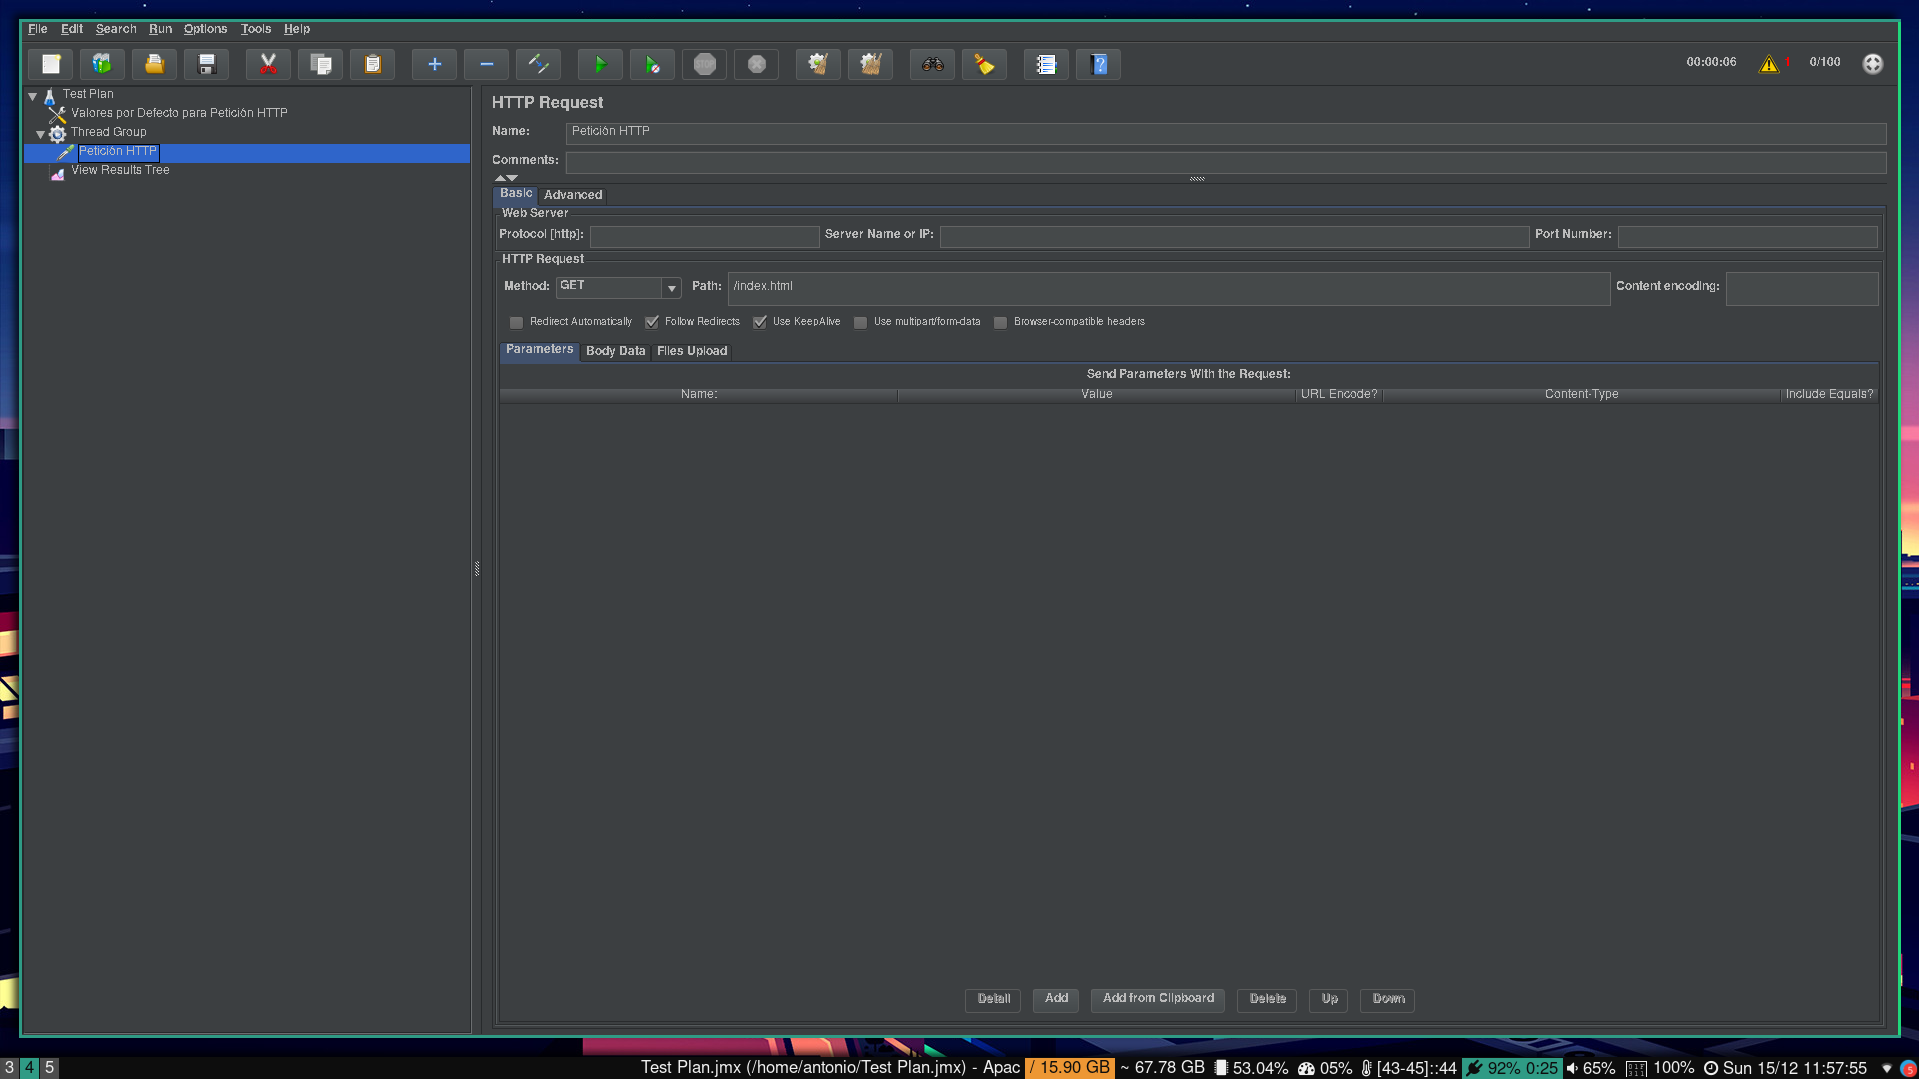
\includegraphics[scale=0.25]{jmeter_basico.png}
\end{center}

\newpage

Al ejecutar vemos como tenemos conexión con el servidor.

\begin{center}
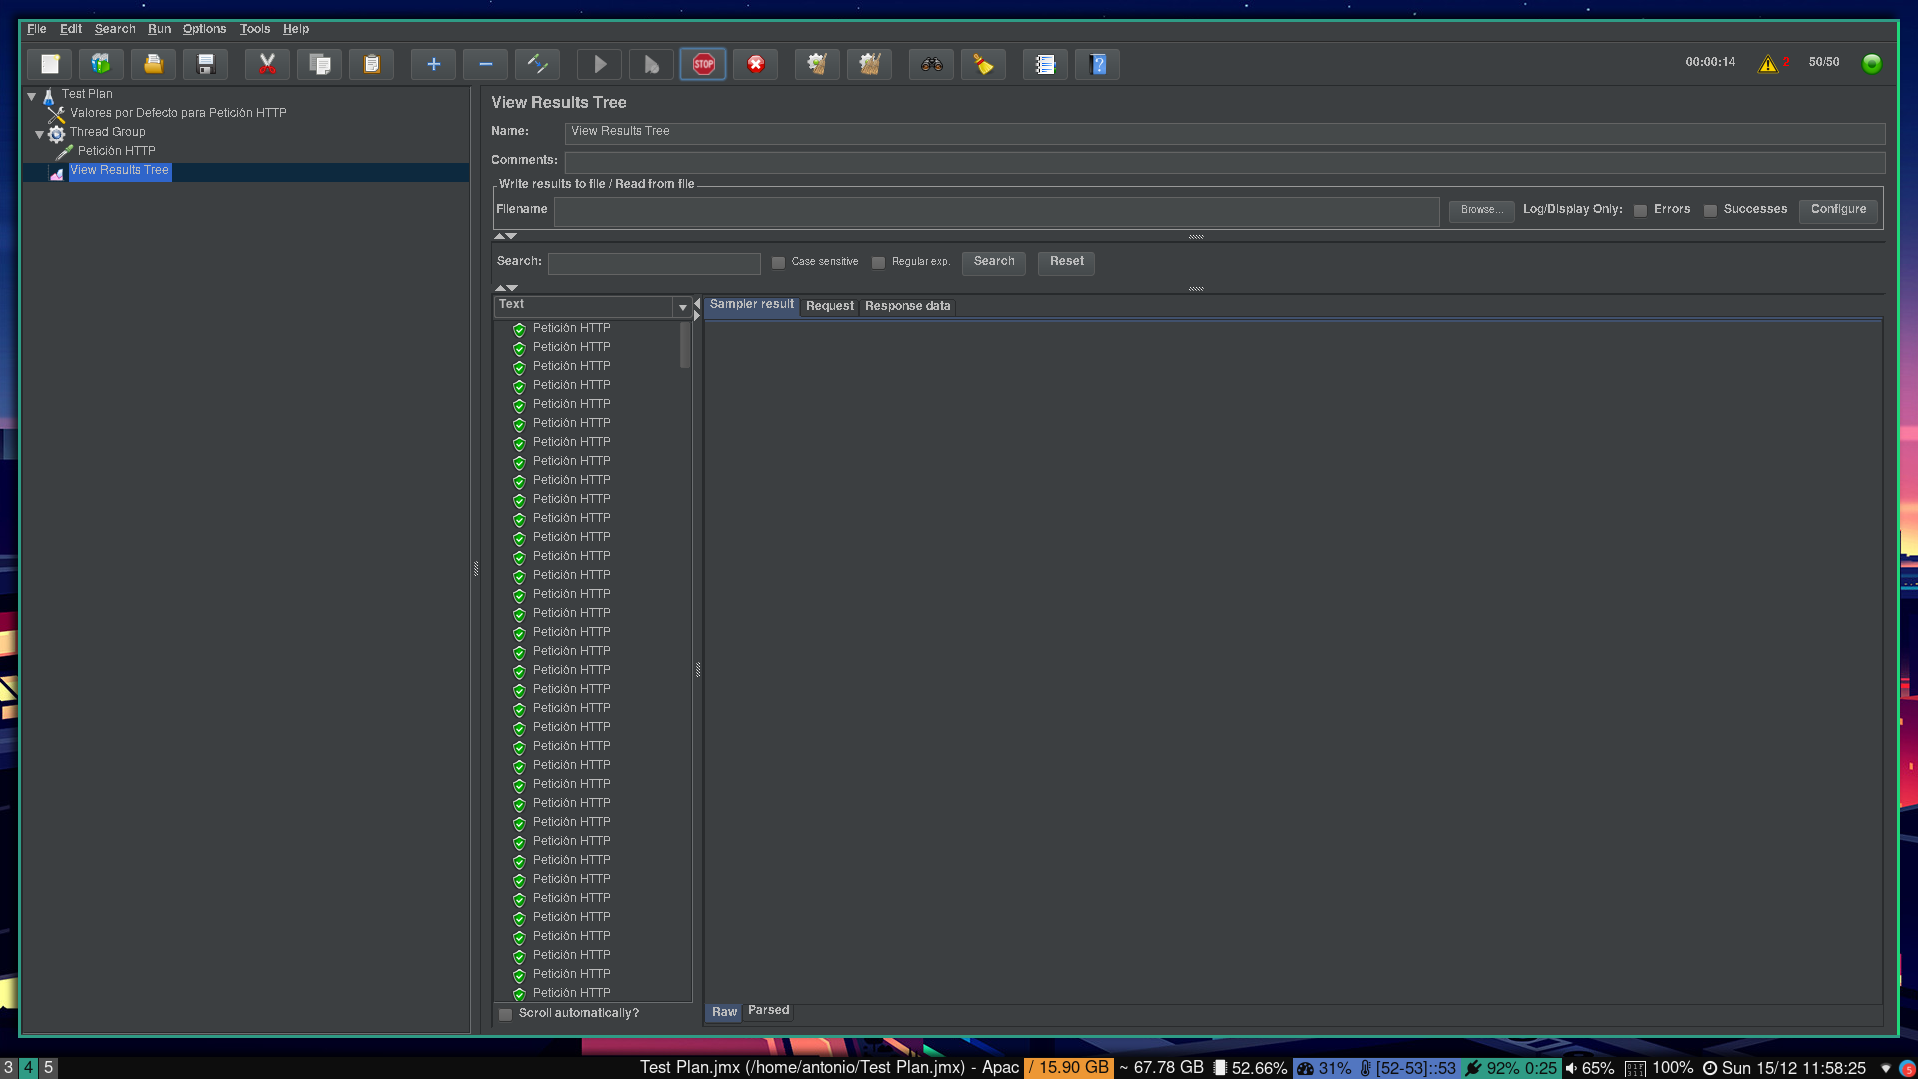
\includegraphics[scale=0.25]{jmeter_p_basico.png}
\end{center}


\newpage

\subsection{Configurando un test de carga para iseP4JMeter}

\subsubsection{Configuración general}

Al igual que con la prueba básica, creamos un elemento de configuración de HTTP, sin embargo, esta vez configuraremos la IP con el valor \texttt{\$\{host\}} y el puerto con \texttt{\$\{puerto\}}. Esto hace referencia a variables, las cuales crearemos en la pestaña del Test, en User Defined Variables. En mi caso estableceré host a \texttt{192.168.56.105} ya que uso Ubuntu para ejecutar el microservicio y como puerto el 3000 porque no he modificado el que venia por defecto.

\begin{center}
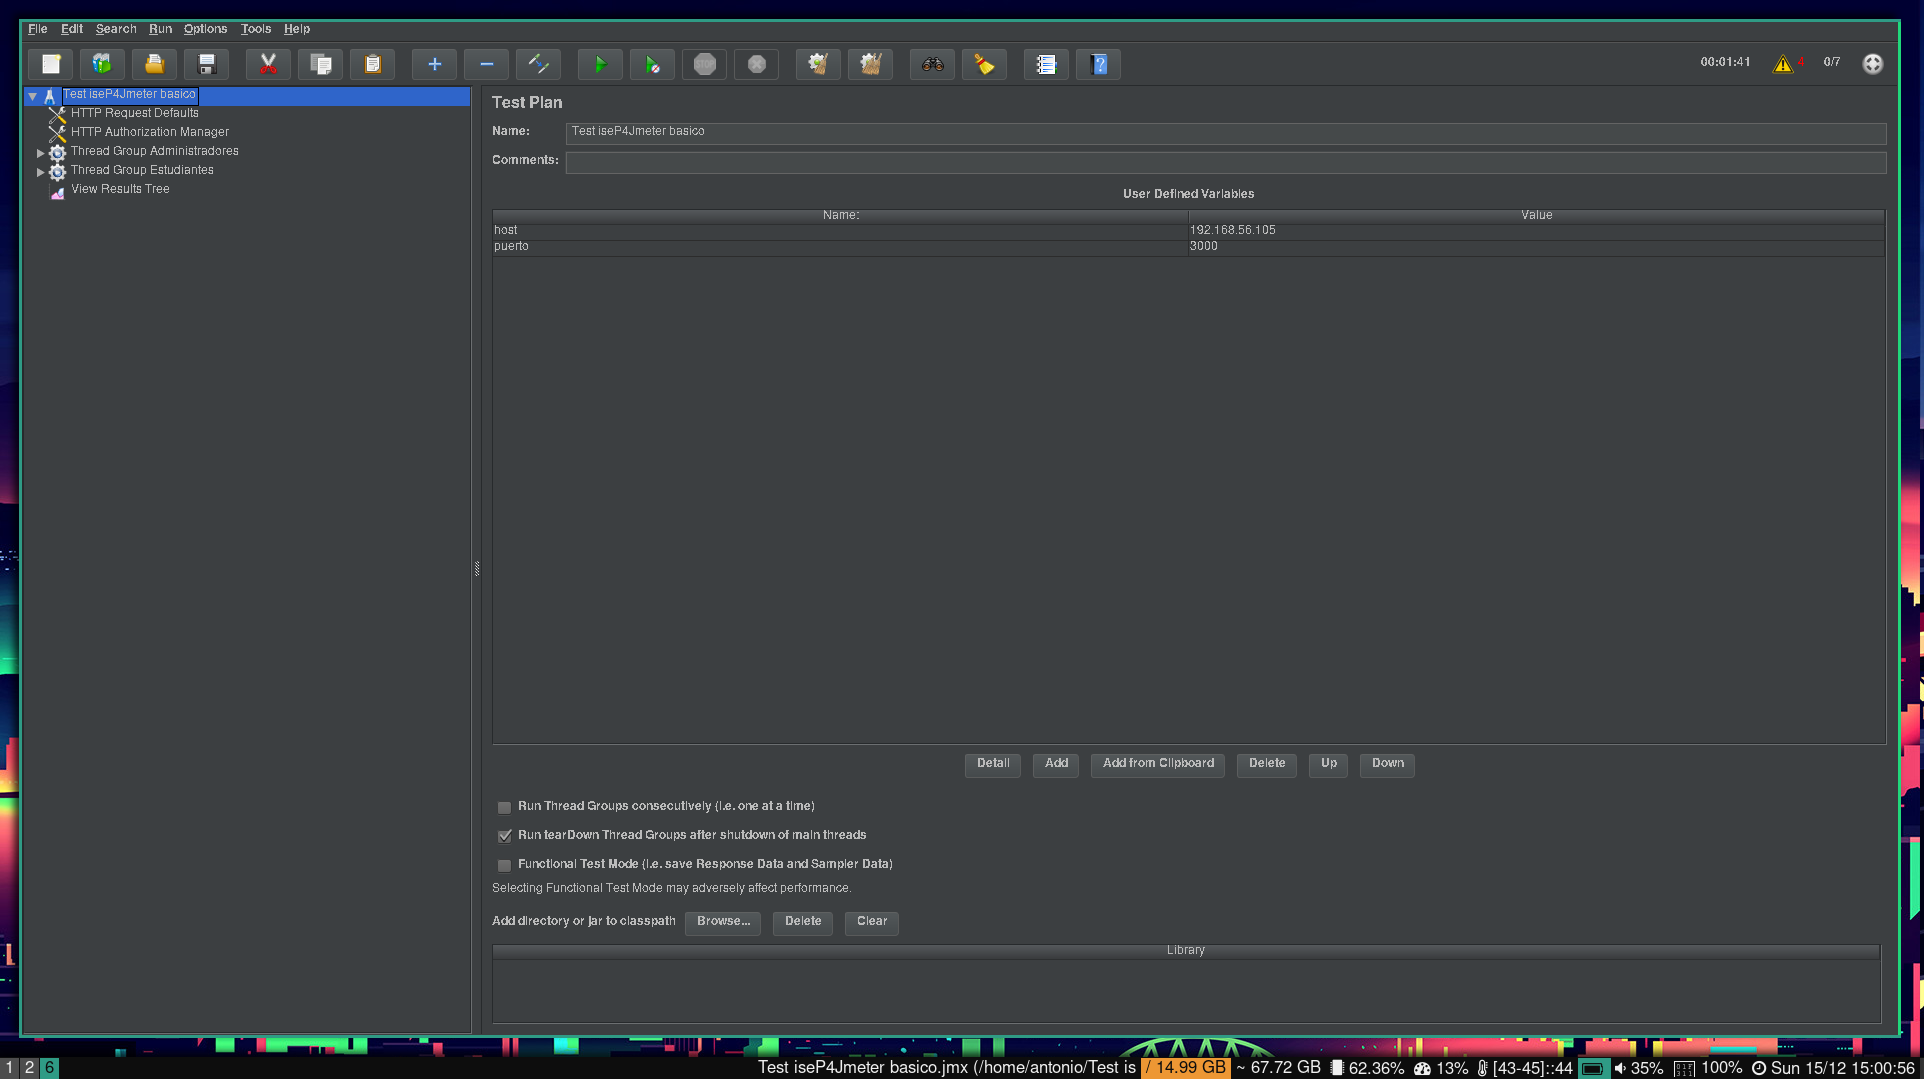
\includegraphics[scale=0.25]{jmeter-1.png}
\end{center}

Como vemos en la imagen también añadimos un elemento de configuración "HTTP Authorization Manager" para gestionar el acceso de BasicAuth, donde añadimos el usuario y clave dados por la aplicación.


\begin{center}
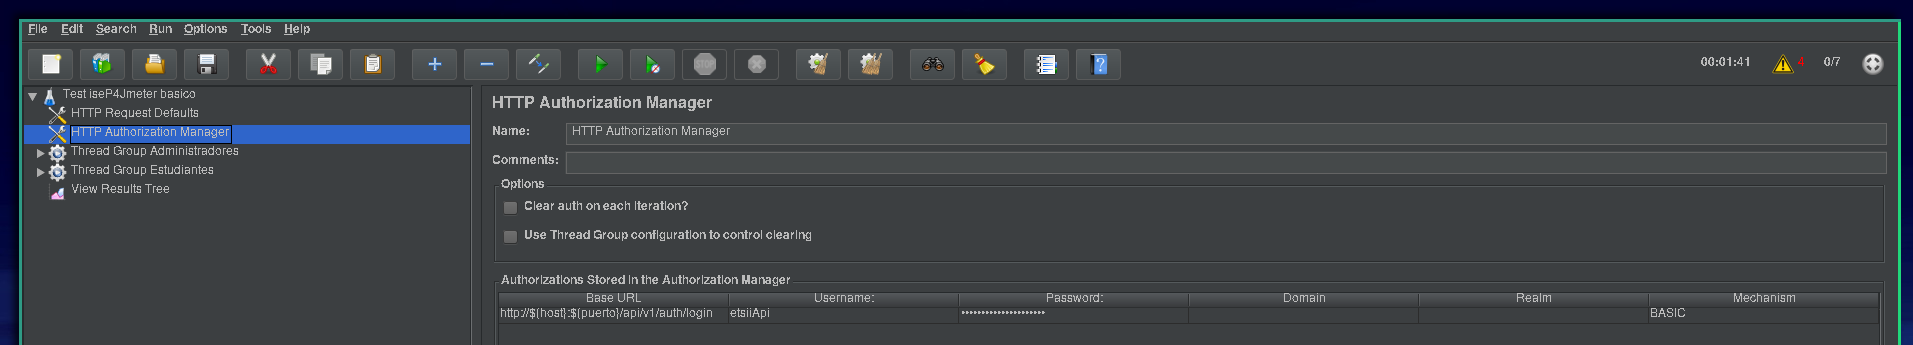
\includegraphics[scale=0.25]{jmeter-2.png}
\end{center}

También añadimos dos Thread Group, uno para estudiantes y otro para administradores, así como un View Results Tree para ver los resultados.


\subsubsection{Configuración para administradores}

Dentro del Thread Group para administradores tenemos que añadir un CSV Data Set Config para que los datos de inicio los tome de un archivo. Dicho archivo tendrá dos columnas, una para el usuario y otra para la contraseña, así que configuramos dos variables en JMeter. También tenemos que seleccionar que ignore la primera fila ya que esta fila es usada para marcar que columna es el usuario y la contraseña.

\begin{center}
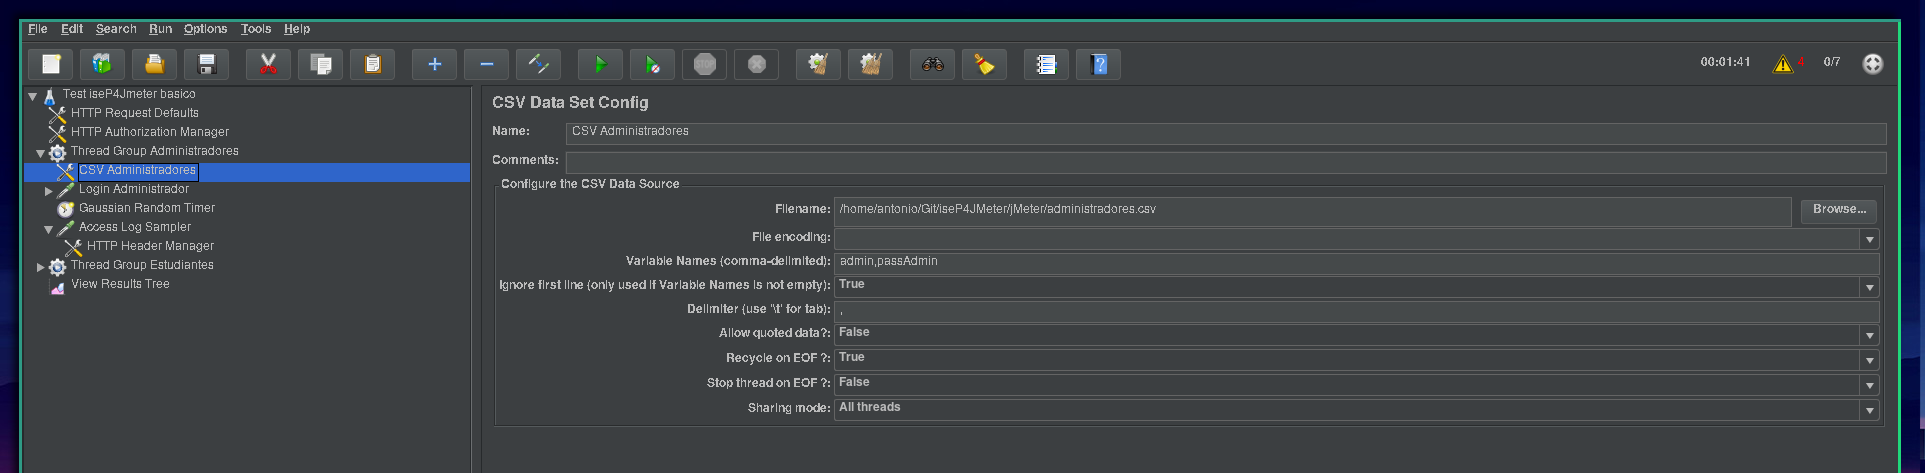
\includegraphics[scale=0.25]{jmeter-3.png}
\end{center}


Crearemos un HTTP Request para que el administrador se inicie sesión. Esta petición será de tipo POST a la ruta \texttt{/api/v1/auth/login}, y le pasaremos dos parámetros, login y password, con los valores recogidos del fichero CSV. El tipo de contenido de estos parámetros será \texttt{application/x-www-form-urlencoded}.

\begin{center}
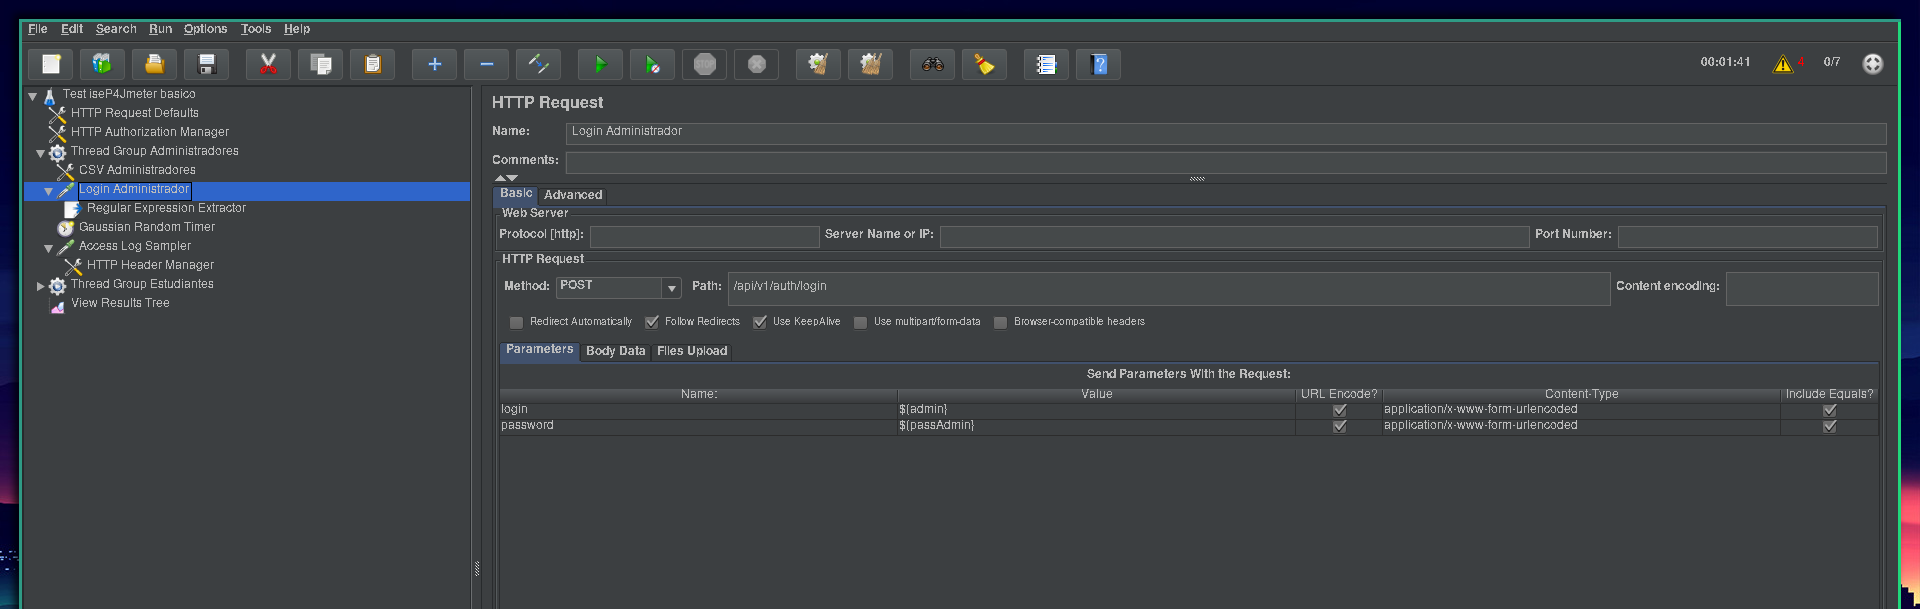
\includegraphics[scale=0.25]{jmeter-4.png}
\end{center}

Una vez hecha la petición de login el servidor nos devolverá el JWT Token del administrador, el cuál usaremos para referirnos a este administrador en futuras peticiones. Almacenaremos este token con un extractor de expresiones regulares, y almacenaremos todo el cuerpo de la respuesta en una variables llamada \texttt{token\_admin}, que más adelante usaremos.

\begin{center}
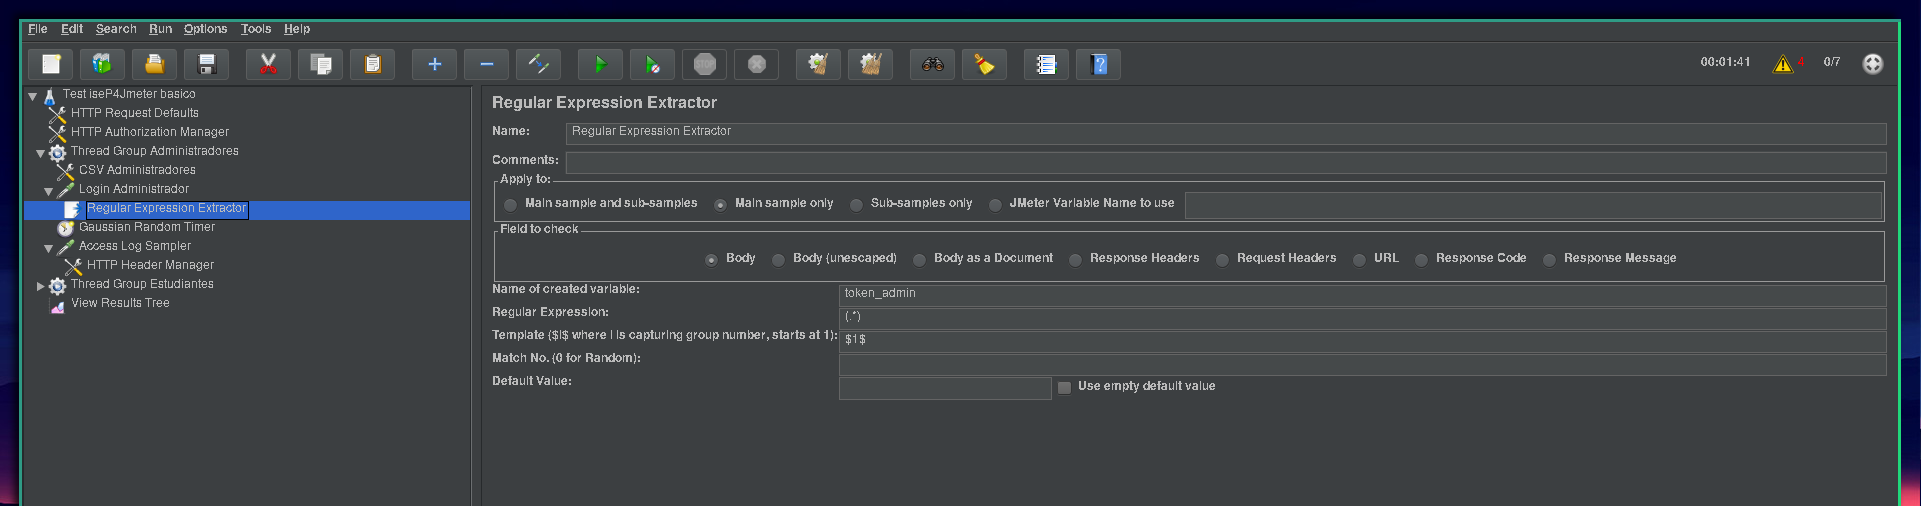
\includegraphics[scale=0.25]{jmeter-5.png}
\end{center}

Como nos pide  el ejercicio, añadimos una espera aleatoria y tras eso añadimos el Access Log Sampler, con el que simularemos el muestreo de acceso de los administradores.

\begin{center}
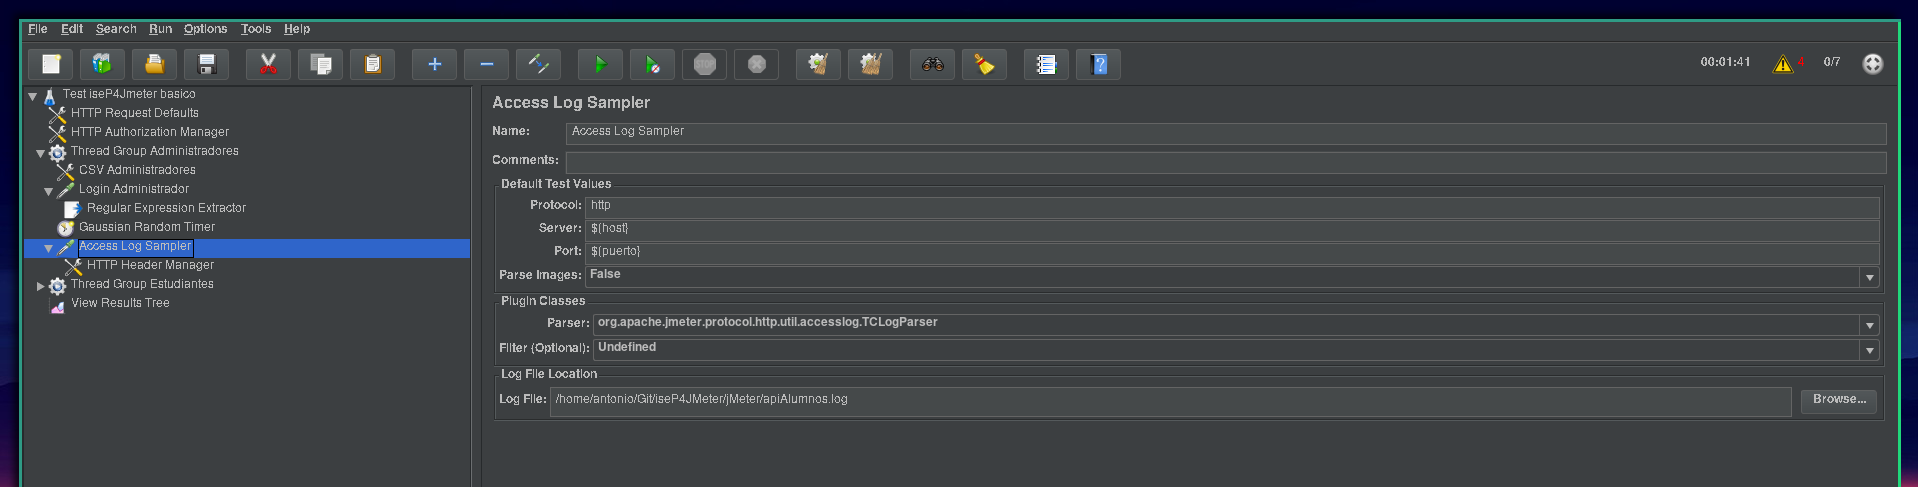
\includegraphics[scale=0.25]{jmeter-6.png}
\end{center}

Para realizar esto, debemos añadir al Access Log Sampler una cabecera de HTTP que adjunte el token obtenido anteriormente.

\begin{center}
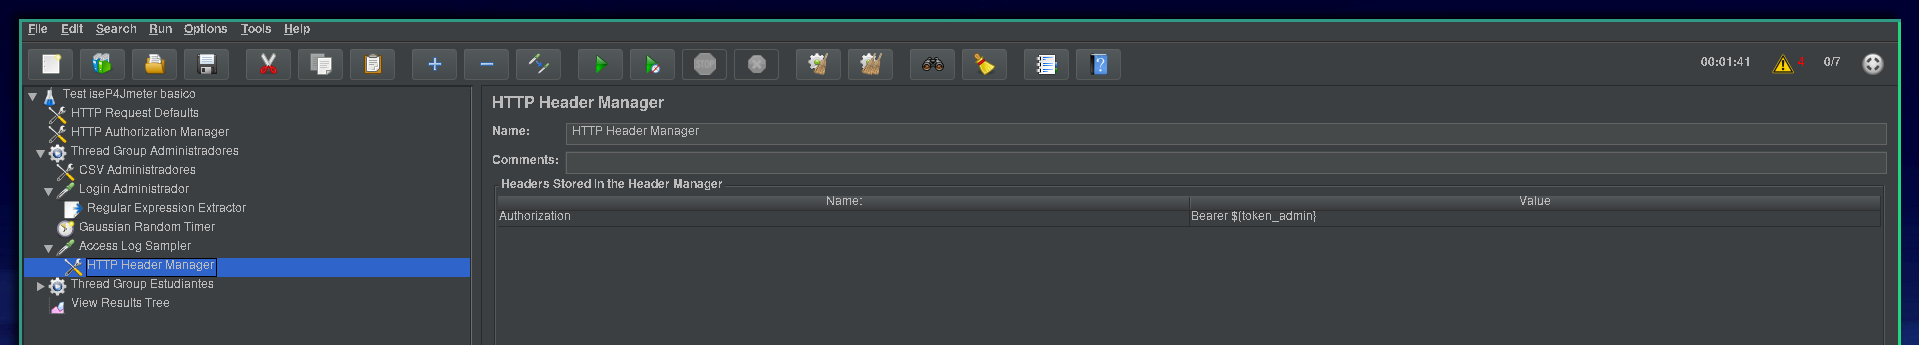
\includegraphics[scale=0.25]{jmeter-7.png}
\end{center}

\subsubsection{Configuración para estudiantes}

Al igual que para los administradores, configuramos el CSV Data Set Config y el login de los estudiantes de la misma forma que para los administradores, solo que usando los datos del archivo alumnos.csv

Además de las opciones de login, debemos añadir una segunda petición HTTP, que en este caso será de tipo GET, con el que obtendremos los datos del estudiante. Pediremos que nos de la ruta \texttt{/api/v1/alumnos/alumno/\$\{user\}}, añadiendo un gestor de cabeceras HTTP que adjunte el token, como hicimos con el Acces Log Sampler del administrador.

\begin{center}
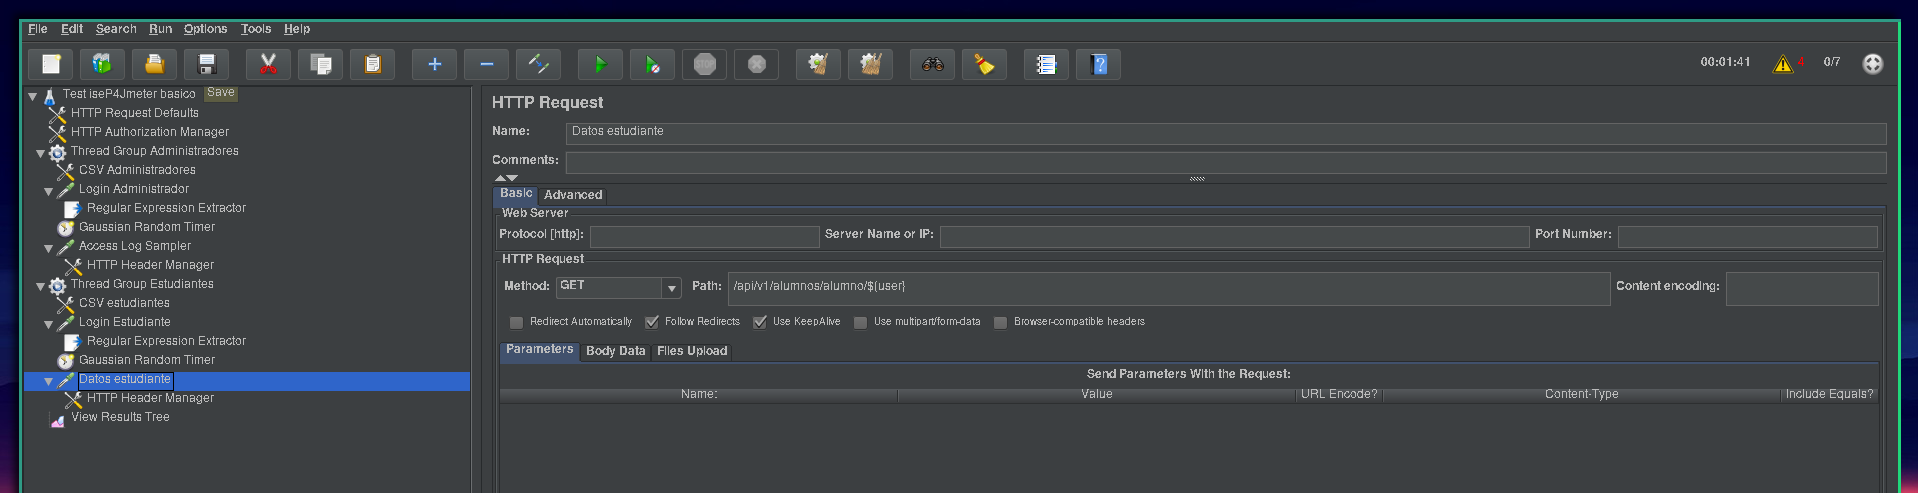
\includegraphics[scale=0.25]{jmeter-8.png}
\end{center}


\begin{center}
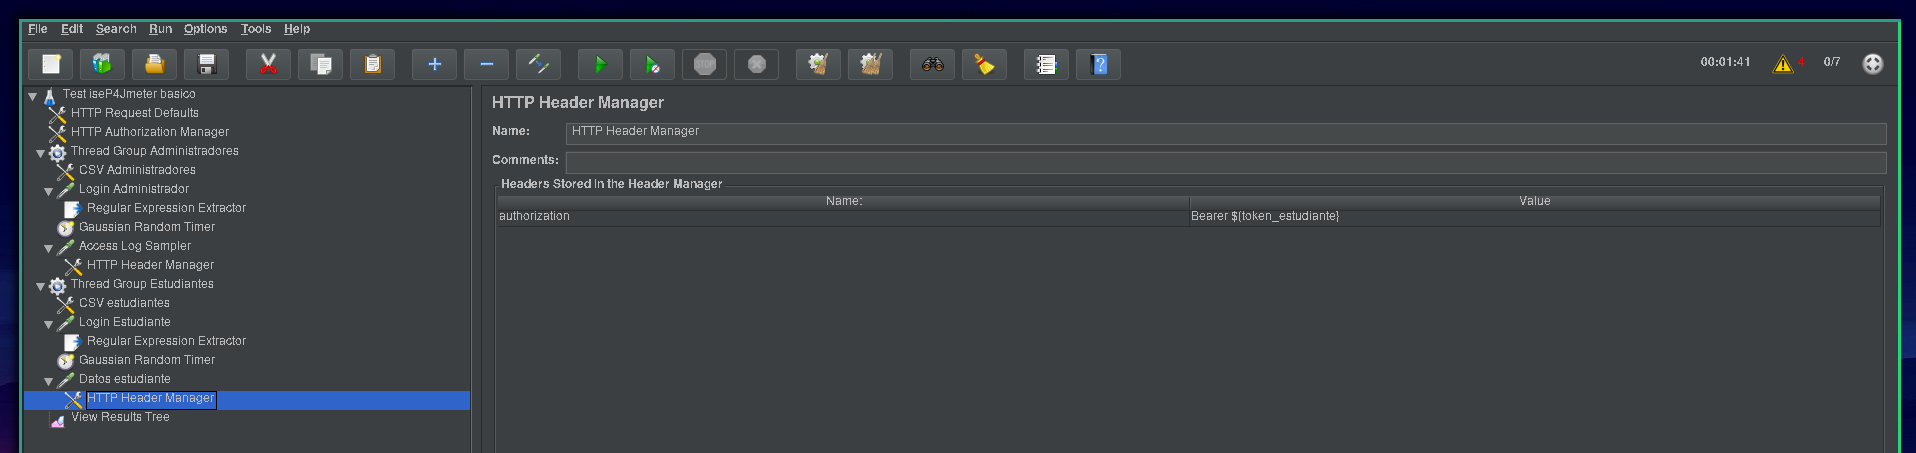
\includegraphics[scale=0.25]{jmeter-9.png}
\end{center}

\subsubsection{Resultados}

Finalmente, si ejecutamos el test de JMeter veremos como todo funciona correctamente.

En mi caso he establecido una única ejecución en los Thread Group por legibilidad.

\begin{center}
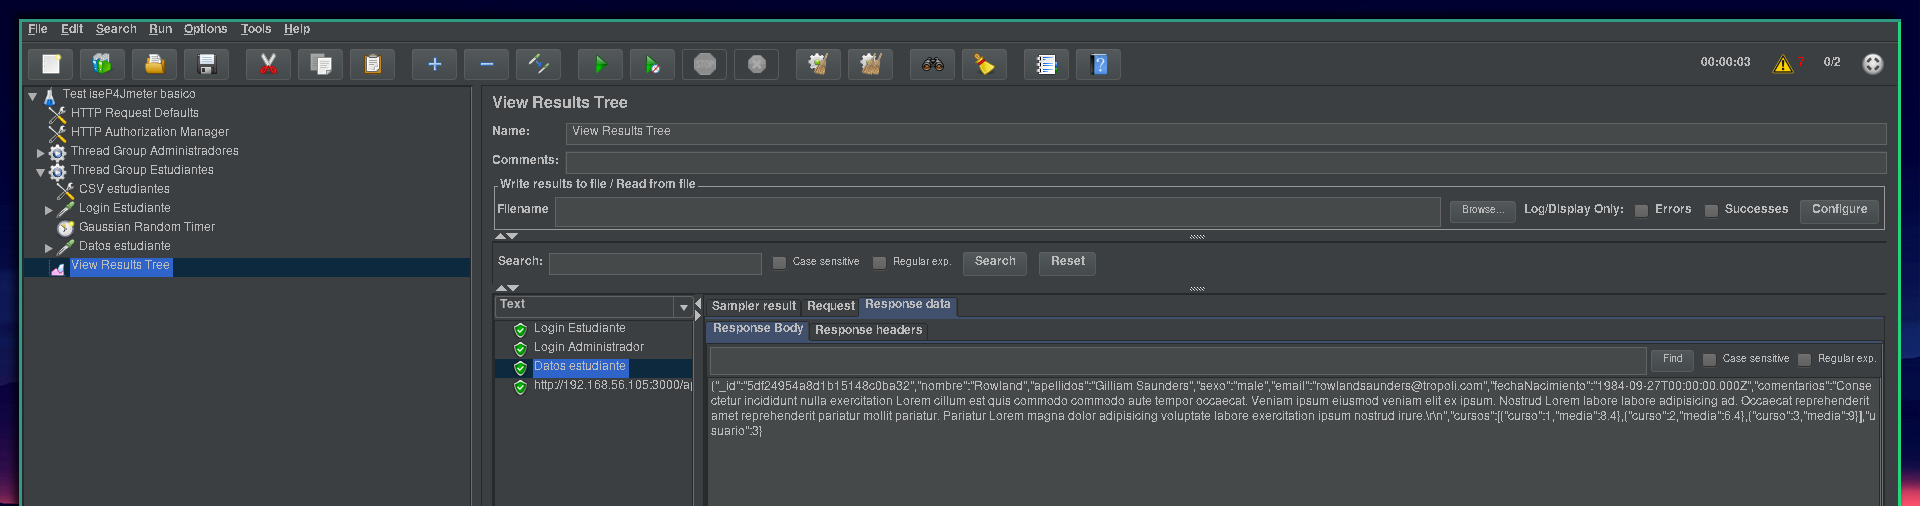
\includegraphics[scale=0.25]{jmeter-10.png}
\end{center}


\newpage

\begin{thebibliography}{9}

\bibitem{pts}
Phoronix Test Suite \url{https://www.phoronix-test-suite.com/}

\bibitem{obm}
OpenBenchmarking \url{https://www.openbenchmarking.org/}

\bibitem{yay}
Yet Another Yogurt (AUR Helper) \url{https://github.com/Jguer/yay}

\bibitem{pts_descarga}
Phoronix Test Suite - Descarga \url{https://www.phoronix-test-suite.com/?k=downloads}

\bibitem{pts_docker}
Docker Phoronix Test Suite \url{https://hub.docker.com/r/phoronix/pts/}

\bibitem{pts_man}
Man phoronix-test-suite \url{https://linux.die.net/man/1/phoronix-test-suite}


\bibitem{ab_doc}
Documentación de AB \url{https://httpd.apache.org/docs/2.4/programs/ab.html}

\bibitem{salida_ab}
Salida de ejecución de AB \url{https://httpd.apache.org/docs/2.4/programs/ab.html#output}

\bibitem{main_jmeter}
Página principal de JMeter \url{https://jmeter.apache.org/}

\bibitem{iseP4JMeter}
Página de iseP4JMeter \url{https://github.com/davidPalomar-ugr/iseP4JMeter}

\bibitem{dockerCentOS}
Instalación de Docker en CentOS \url{https://docs.docker.com/v17.09/engine/installation/linux/docker-ce/centos/#set-up-the-repository}

\end{thebibliography}


\end{document}
